\documentclass[a4paper]{article}
\usepackage[margin=3.5cm, marginparsep=5pt, marginparwidth=80pt]{geometry}
\usepackage{amsmath}
\usepackage{amssymb}
\usepackage[svgnames,rgb]{xcolor}
\usepackage{amsthm}
% \makeatletter
% \def\th@plain{%
%   \thm@notefont{}% same as heading font
%   \itshape % body font
% }
% \def\th@definition{%
%   \thm@notefont{}% same as heading font
%   \normalfont % body font
% }
% \makeatother
\usepackage{dsfont}
\usepackage{graphicx}
\usepackage{caption}
\usepackage{hyperref}
\usepackage{cleveref}
\usepackage{datetime}
\usepackage{outlines}
\usepackage{float}
\usepackage{booktabs}
\usepackage{enumitem}
\usepackage{tabto}
\usepackage{mathtools}
\usepackage{nicematrix}
\usepackage{nccmath}

\usepackage{algorithm}
\usepackage{algpseudocode}

\usepackage{lipsum}
\usepackage{pdfcomment}
\usepackage[activate={true,nocompatibility},final,tracking=true,kerning=true,spacing=true,factor=500,stretch=15,shrink=15]{microtype}

\usepackage{apptools}
\AtAppendix{\counterwithin{lemma}{section}}

\addtolength{\skip\footins}{2mm}

\newcommand{\comment}[1]{\pdfmargincomment[author=Jeroen van Riel]{#1}}

% code highlighting
\usepackage{minted}
\usepackage{xpatch}
\newminted[cminted]{python}{fontsize=\small}
\xpretocmd{\cminted}{\RecustomVerbatimEnvironment{Verbatim}{BVerbatim}{}}{}{}

% link coloring
\hypersetup{
   colorlinks,
   linkcolor={red!90!black},
   citecolor={green!40!black},
   urlcolor={blue!60!black}
}

% concatenation symbol (c.f. ++ in Haskell)
\newcommand\mdoubleplus{\mathbin{+\mkern-10mu+}}

% end of proof symbol
\newcommand{\newmarkedtheorem}[1]{%
  \newenvironment{#1}
    {\pushQED{\qed}\csname inner@#1\endcsname}
    {\popQED\csname endinner@#1\endcsname}%
  \newtheorem{inner@#1}%
}
% \renewenvironment{proof}{{\noindent\bfseries Proof.}}{*something*}
% \let\oldproofname=\proofname
% \renewcommand{\proofname}{\rm\bf{\oldproofname}}

\theoremstyle{definition}
%\newtheorem{eg}{Example}[section]
\newmarkedtheorem{eg}{Example}[section]
\newtheorem{define}{Definition\hspace{0.25em}\ignorespaces}
\newtheorem{remark}{Remark}
\theoremstyle{plain}
\newtheorem{property}{Property\hspace{0.25em}\ignorespaces}
\newtheorem{observation}{Observation}
\newtheorem{proposition}{Proposition}
\newtheorem{lemma}{Lemma\hspace{0.25em}\ignorespaces}
\newtheorem{corollary}{Corollary}
\newtheorem{theorem}{Theorem\hspace{0.25em}\ignorespaces}
\newtheorem{assump}{Assumption\hspace{0.25em}\ignorespaces}

\DeclareMathOperator{\interior}{int}
\DeclareMathOperator*{\argmax}{arg\,max}
\DeclareMathOperator*{\argmin}{arg\,min}
\newcommand*\diff{\mathop{}\!\mathrm{d}}

% cref settings
\crefname{equation}{equation}{equations}
\newcommand{\crefrangeconjunction}{--}

\newdateformat{monthyeardate}{\monthname[\THEMONTH] \THEYEAR}

\author{Jeroen van Riel}
\date{\monthyeardate\today}

\title{Vehicle trajectory planning in a single lane with minimum following
  distance and boundary conditions}

\begin{document}

\maketitle

\begin{abstract}
  We study a model for a single-lane road where overtaking is not permitted.
  %
  Vehicles are modeled as double integrators, i.e., position and speed are
  governed by acceleration control, subject to bounds on speed and acceleration.
  Consecutive vehicles must maintain a fixed following distance to avoid
  collisions.
  %
  Each vehicle has predetermined times for entry and exit, both of which must
  occur at full speed.
  %
  For the objective of minimizing distance to the end of the lane over time, we
  present an algorithm to compute optimal trajectories.
  %
  Assuming a fixed minimum lane length, we characterize the feasibility of this
  trajectory planning problem through a system of linear inequalities that
  depend only on the schedule times.
  %
\end{abstract}

% \tableofcontents

\newcommand\halfopen[2]{\ensuremath{[#1,#2)}}
\newcommand\openhalf[2]{\ensuremath{(#1,#2]}}

\renewcommand{\labelitemii}{\textbullet}
\renewcommand{\labelitemiii}{\textbullet}

\newcommand\note[1]{{\color{Navy}#1}}

\section{Optimal control formulation of isolated lane model}

We will propose a model for a one-directional single-lane road of finite length
where overtaking is not permitted.
%
We will link such lanes together to construct a model representing a
network of intersections.
%
The fact that a lane between two intersections is of limited length---unlike the
approaching lanes of the isolated intersection model---means that it can be
occupied by a limited number of vehicles at the same time.
%
This property makes the characterization of set of feasible trajectories more
involved.

% feasibility analysis (of safe sets of trajectories)
Given some lane, consider the set of vehicles that need to travel across this
lane as part of their planned route. Suppose that the time of entry to and exit
from this lane are fixed for each of these vehicles, then the question is
whether there exists a set of trajectories that is safe, i.e.\ without
collisions, and satisfies these \emph{schedule times}.
%
Loosely speaking, we want an easy way to answer this question for any set of
schedule times.
%
By requiring vehicles to enter and exit the lane at \emph{full speed}, we will
show that this feasibility question is precisely answered by a system of linear
inequalities in terms of the schedule times.

% optimal control problem
% byproduct: algorithm for bang-bang solutions
Because there is generally not a single feasible set of trajectories, we can
consider some performance criterion, for example by measuring some sort of
smoothness to model passenger comfort or energy consumption.
%
The resulting optimal control problem is straightforward to solve using a direct
transcription method.
%
However, when we seek to minimize each vehicle's distance
to the end of the lane at all times, to which we refer as the \emph{haste
  objective}, we will show that the optimal solution can be computed much more
efficiently.
%
We will see that the derivation of this algorithm is a direct byproduct of the
feasibility analysis, because the latter will involve the construction of a
certain set of upper bounding trajectories, which happen to be optimal under the
haste objective.

In the remainder of this introducion, we will precisely establish the notion of
a feasible set of trajectories in a lane. After precisely defining the optimal
control problem under study, we show some examples of feasible trajectories for
the haste objective and for the minimization of some proxy for energy
consumption.


\paragraph{Vehicle trajectories.}
We only consider the longitudinal position of vehicles on the lane and we assume
that speed and acceleration are bounded. Therefore, let $\mathcal{D}[a,b]$
denote the set of valid \emph{trajectories}, which we define to be all continuously
differentiable functions $x : [a,b] \rightarrow \mathbb{R}$ satisfying the constraints
\begin{align}
  0 \leq \dot{x}(t) \leq 1 \quad \text{ and } \quad
  {-\omega} \leq \ddot{x}(t) \leq \bar{\omega} , \quad \text{ for all } t \in [a,b] ,
\end{align}
for some fixed acceleration bounds $\omega, \bar{\omega} > 0$ and with $\dot{x}$ and
$\ddot{x}$ denoting the first and second derivative with respect to time $t$.
Note that the unit speed upper bound is not restrictive, since we can always
apply an appropriate scaling of time and the acceleration bounds to arrive at
this form.
%
We use $A$ and $B$ to denote the start\footnote{Note that assuming $A\neq 0$ is convenient later when we start piecing together multiple lanes.} and end position of the lane.
%
Let $D_{1}[a, b] \subset \mathcal{D}[a, b]$ denote all trajectories $x$ that satisfy
the first-order boundary conditions
\begin{align}
  x(a) = A \; \text{ and } \; x(b) = B .
\end{align}
Additionally, let $D_{2}[a,b] \subset D_{1}[a, b]$ further induce the second-order
boundary conditions
\begin{align}
  \dot{x}(a) = \dot{x}(b) = 1 .
\end{align}
In words, these boundary conditions require that a vehicle arrives to and
departs from the lane at predetermined times $a$ and $b$ and do so at full
speed.
%
Figure~\ref{fig:trajectories} shows an example for each of these three classes of trajectories.


\begin{figure}
  \centering
  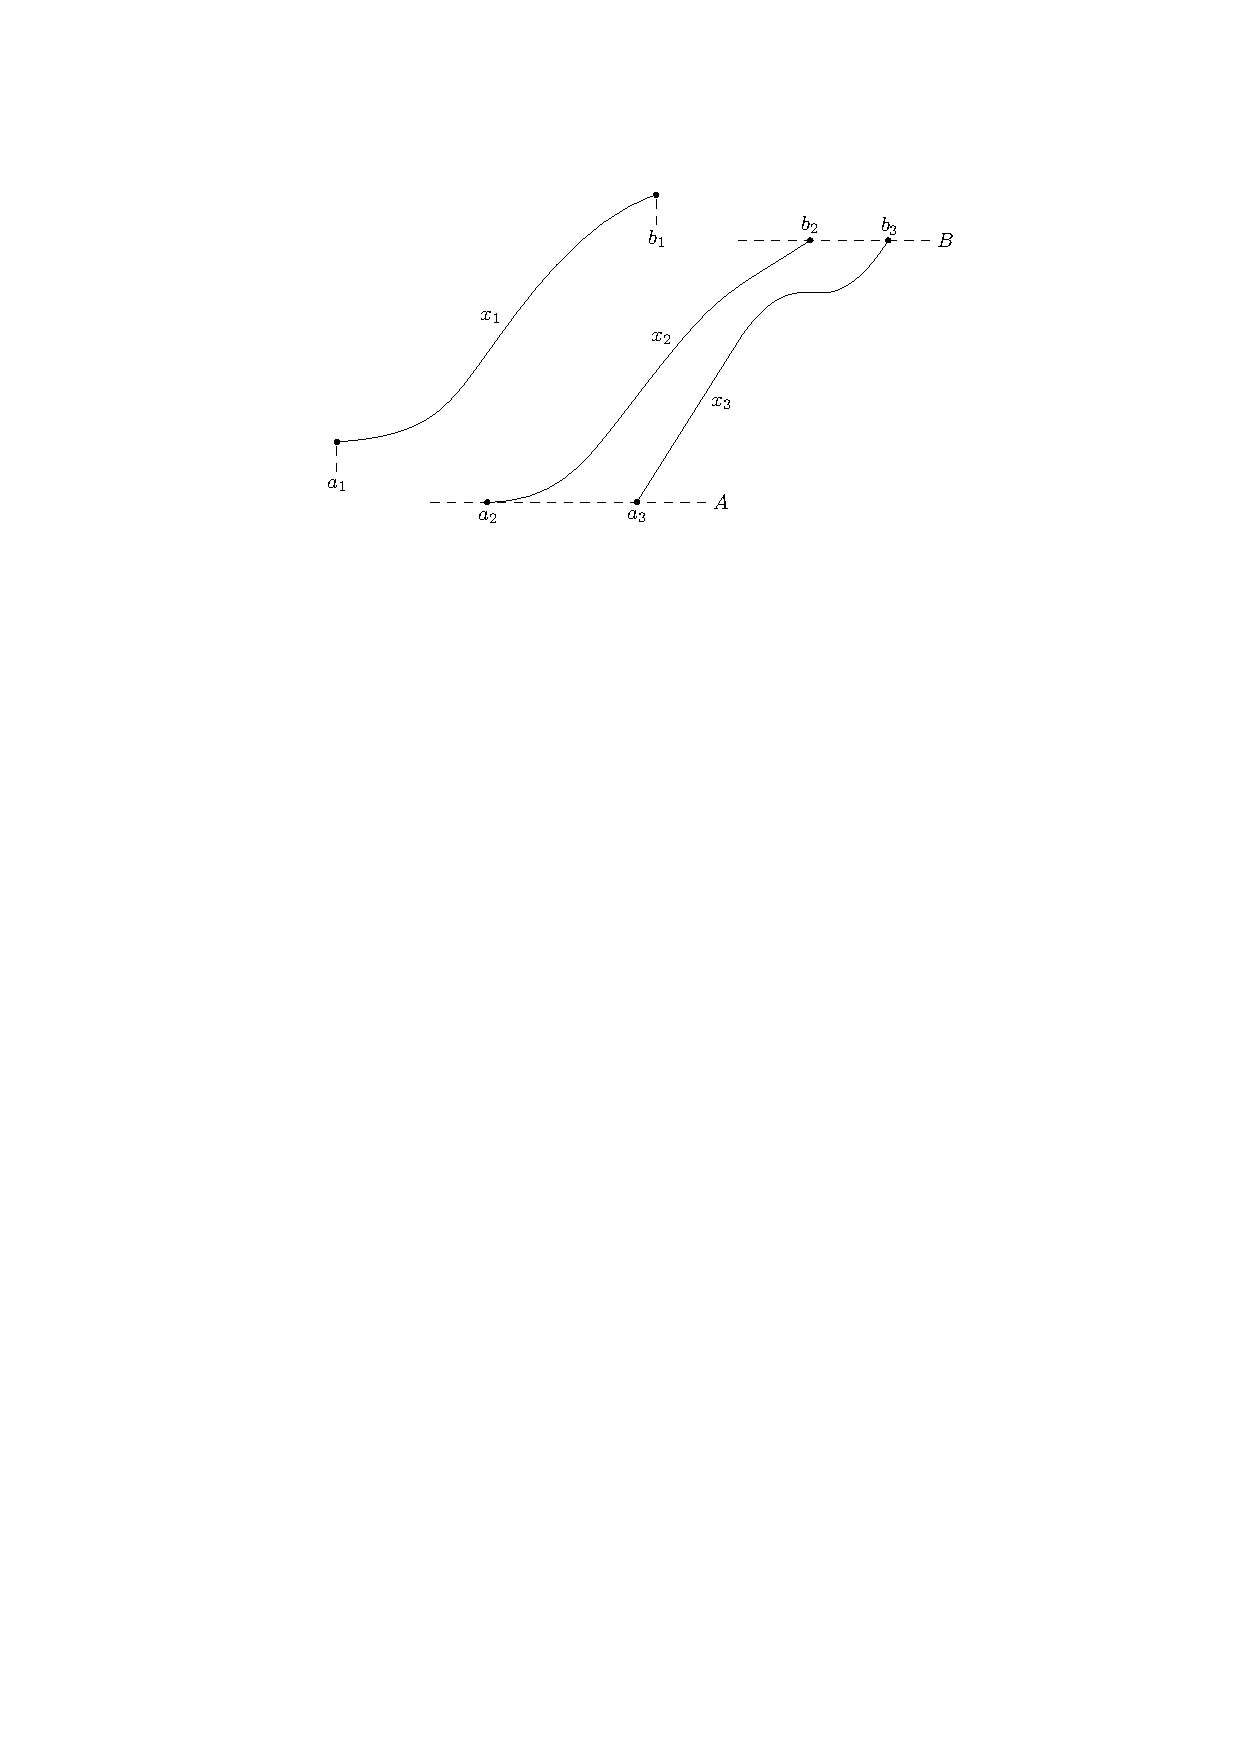
\includegraphics[scale=0.9]{figures/motion/trajectories}
  \caption{Example trajectories $x_{1} \in \mathcal{D}[a_{1},b_{1}]$,
    $x_{2} \in D_{1}[a_{2},b_{2}]$ and $x_{3} \in D_{2}[a_{3},b_{3}]$ for each the
    three classes of trajectories that are used throughout this chapter.}%
  \label{fig:trajectories}
\end{figure}

\paragraph{Trajectory domains.}
Function domains will play an important role in the analysis of feasible
trajectories. Therefore, we introduce some useful notational conventions.
%
First of all, each of the trajectory classes above can be used with the common
convention of allowing $a = -\infty$ or $b = \infty$. For instance, we write
$\mathcal{D}(-\infty, \infty)$ to denote the set of trajectories defined on the
whole real line.
%
Furthermore, we use $\cdot\,|_{[a,b]}$ to denote function restriction. For example,
\begin{align*}
  (t \mapsto t + 1)|_{\halfopen{\xi}{\infty}}
\end{align*}
denotes some anonymous function with some restricted domain.
%
Furthermore, given two smooth trajectories $\gamma_{1} \in \mathcal{D}[a_{1}, b_{1}]$
and $\gamma_{2} \in \mathcal{D}[a_{2}, b_{2}]$, we write inequality
  $\gamma_{1} \preceq \gamma_{2}$ to mean
\begin{align*}
\gamma_{1}(t) \leq \gamma_{2}(t) \; \text{ for all } \; t \in [a_{1}, b_{1}] \cap [a_{2}, b_{2}] .
\end{align*}
%
Whenever the intersection of domains is empty, we say that the above inequality
is \emph{void}.
%
The reason for introducing a dedicated symbol is that $\preceq$ is not transitive.
To see this, consider the trajectories in Figure~\ref{fig:trajectories}, then
$x_{1} \preceq x_{3}$ (void) and $x_{3} \preceq x_{2}$, but clearly
$x_{1} \npreceq x_{2}$.

\begin{define}
  Let $L > 0$ denote the \textit{following distance} between consecutive vehicles.
  %
  Suppose there are $N$ vehicles scheduled to traverse the lane. For each
  vehicle $i$, let $a_{i}$ and $b_{i}$ denote the \textit{schedule time} for entry and
  exit, respectively.
  %
  Assuming that the schedule times are ordered as
  $a_{1} \leq a_{2} \leq \dots \leq a_{N}$ and
  $b_{1} \leq b_{2} \leq \dots \leq b_{N} $, then a \emph{feasible solution} consists
  of a sequence of trajectories $x_{1}, \dots, x_{N}$ such that
\begin{subequations}\label{eq:feasibility}
\begin{align}
x_{i} \in D_{2}[a_{i}, b_{i}] \quad \quad & \text{ for each } i \in \{1, \dots, N\}, \label{eq:second-order-constraint} \\
x_{i} \preceq x_{i-1} - L \quad \quad & \text{ for each } i \in \{2, \dots, N\} . \label{eq:lead-constraint}
\end{align}
\end{subequations}
We will refer to~\eqref{eq:lead-constraint} as the \emph{lead vehicle
  constraints}.
%
For some performance criterion of trajectories, given as a functional $J(x)$ of
trajectory $x$, the \emph{lane planning problem} is to find a feasible solution that
maximizes
\begin{align}\label{eq:objective}
  \max \; \sum_{i=1}^{N} J(x_{i}) .
\end{align}
\end{define}

We emphasize again that~\eqref{eq:second-order-constraint} requires vehicles to
enter and exit the lane at full speed.
%
The feasibility characterization that we will derive can now be roughly stated
as follows. Assuming the system parameters $(\omega, \bar{\omega},A,B,L)$ to be
fixed, with lane length $B-A$ sufficiently large and following distance $L$
sufficiently small, feasibility of the lane planning problem is characterized by
a system of linear inequalities in terms of the schedule times $a_{i}$ and
$b_{i}$.

\paragraph{Choice of objective.}
We obtain what we call the \emph{haste objective} by choosing
\begin{align}\label{eq:haste-objective}
  J(x_{i}) = \int_{a_{i}}^{b_{i}} x_{i}(t) \diff t .
\end{align}
%
Roughly speaking, this objective seeks to keep all vehicles as close to the end
of the lane at all times, but it does not capture energy efficiency in any way.
%
\note{Introduce energy objective and present some examples for both for comparison.}
%
In the rest of this chapter, we will show that optimal trajectories under the
haste objective can be understood as the concatenation of at most four different
types of trajectory parts, which we might call \emph{bang-off-bang}. Based on
this observation, we present an algorithm to compute optimal trajectories.
%
Extending this algorithm to objectives like \note{[the energy objective]}, is an
interesting topic for further research.

% \subsection{Direct transcription}

% A straightforward way of solving
% problem~\eqref{eq:feasibility}--\eqref{eq:objective} is through direct
% transcription to a mixed-integer linear program by only considering the vehicle
% trajectories $x_{i}(t)$ at discrete time steps $t_{1}, t_{2}, \dots, t_{n}$.
% %
% We can use the forward Euler scheme to discretize the constraints.
% %
% The downside of this technique is that its computational complexity scales very
% poorly with the number of time steps.

\section{Single vehicle with arbitary lead vehicle constraint}

Before we analyze the feasibility of the lane planning problem as a whole, we
focus on the lead vehicle constraint~\eqref{eq:lead-constraint} for a single
vehicle $i \geq 2$.
%
This allows us to lighten the notation slightly by dropping the vehicle index
$i$. Instead of $x_{i-1} - L$, we assume we are given some arbitrary \emph{lead vehicle boundary}
$u$ and consider the following problem.

\begin{define}
  Let $u \in D_{1}[c, d]$ and assume we are given two schedule times
  $a,b \in \mathbb{R}$ such that $a \geq c$ and $b \geq d$, then the
  \emph{single vehicle (feasibility) problem} is to find a trajectory
  \begin{align}
    x \in D_{2}[a,b] \; \text{ such that } \; x \preceq u .
  \end{align}
\end{define}

\subsection{Necessary conditions}

Suppose we are given some feasible trajectory $x \in D_{2}[a,b]$.
%
In addition to the given upper bounding trajectory $u$, we will derive two
upper bounding trajectories $x^{1}$ and $\hat{x}$ and one lower bounding
trajectory $\check{x}$, see Figure~\ref{fig:necessary-conditions}.
%
Using these bounding trajectories, we will formulate four necessary conditions
for the single vehicle problem.

Let the \emph{full speed boundary}, denoted $x^{1}$, be defined as
\begin{align}
  x^{1}(t) = A + t - a,
\end{align}
for all $t \in [a, b]$, then we clearly have $x \preceq x^{1}$.
%
Next, since deceleration is at most $\omega$, we have
$\dot{x}(t) \geq \dot{x}(a) - \omega(t - a) = 1 - \omega(t - a)$, which we
combine with the speed constraint $\dot{x} \geq 0$ to derive
$\dot{x}(t) \geq \max\{0, 1 - \omega (t - a) \}$. Hence, we obtain the lower
bound
\begin{align}\label{eq:check-x}
  x(t) = x(a) + \int_{a}^{t} \dot{x}(\tau) \diff \tau \geq A + \int_{a}^{t} \max\{0, 1 - \omega (\tau - a) \} \diff \tau =: \check{x}(t) ,
\end{align}
for all $t \geq a$, so that we have $x \succeq \check{x}$.
%
Analogously, we derive an upper bound from the fact that acceleration is at most $\bar{\omega}$. Observe that we have
$\dot{x}(t) + \bar{\omega} (b - t) \geq \dot{x}(b) = 1$, which we combine
with the speed constraint $\dot{x}(t) \geq 0$ to derive
$\dot{x}(t) \geq \max \{ 0, 1 - \bar{\omega}(b - t) \}$. Hence, we obtain the
upper bound
\begin{align}\label{eq:hat-x}
  x(t) = x(b) - \int_{t}^{b} \dot{x}(\tau) \diff \tau
  \leq B - \int_{t}^{b} \max\{ 0, 1 -\bar{\omega} (b - \tau) \} \diff \tau =: \hat{x}(t) ,
\end{align}
for all $t \leq b$, so we have $x \preceq \hat{x}$.
%
We refer to $\check{x}$ and $\hat{x}$ as the \emph{entry boundary} and
\emph{exit boundary}, respectively.

\begin{figure}
  \centering
  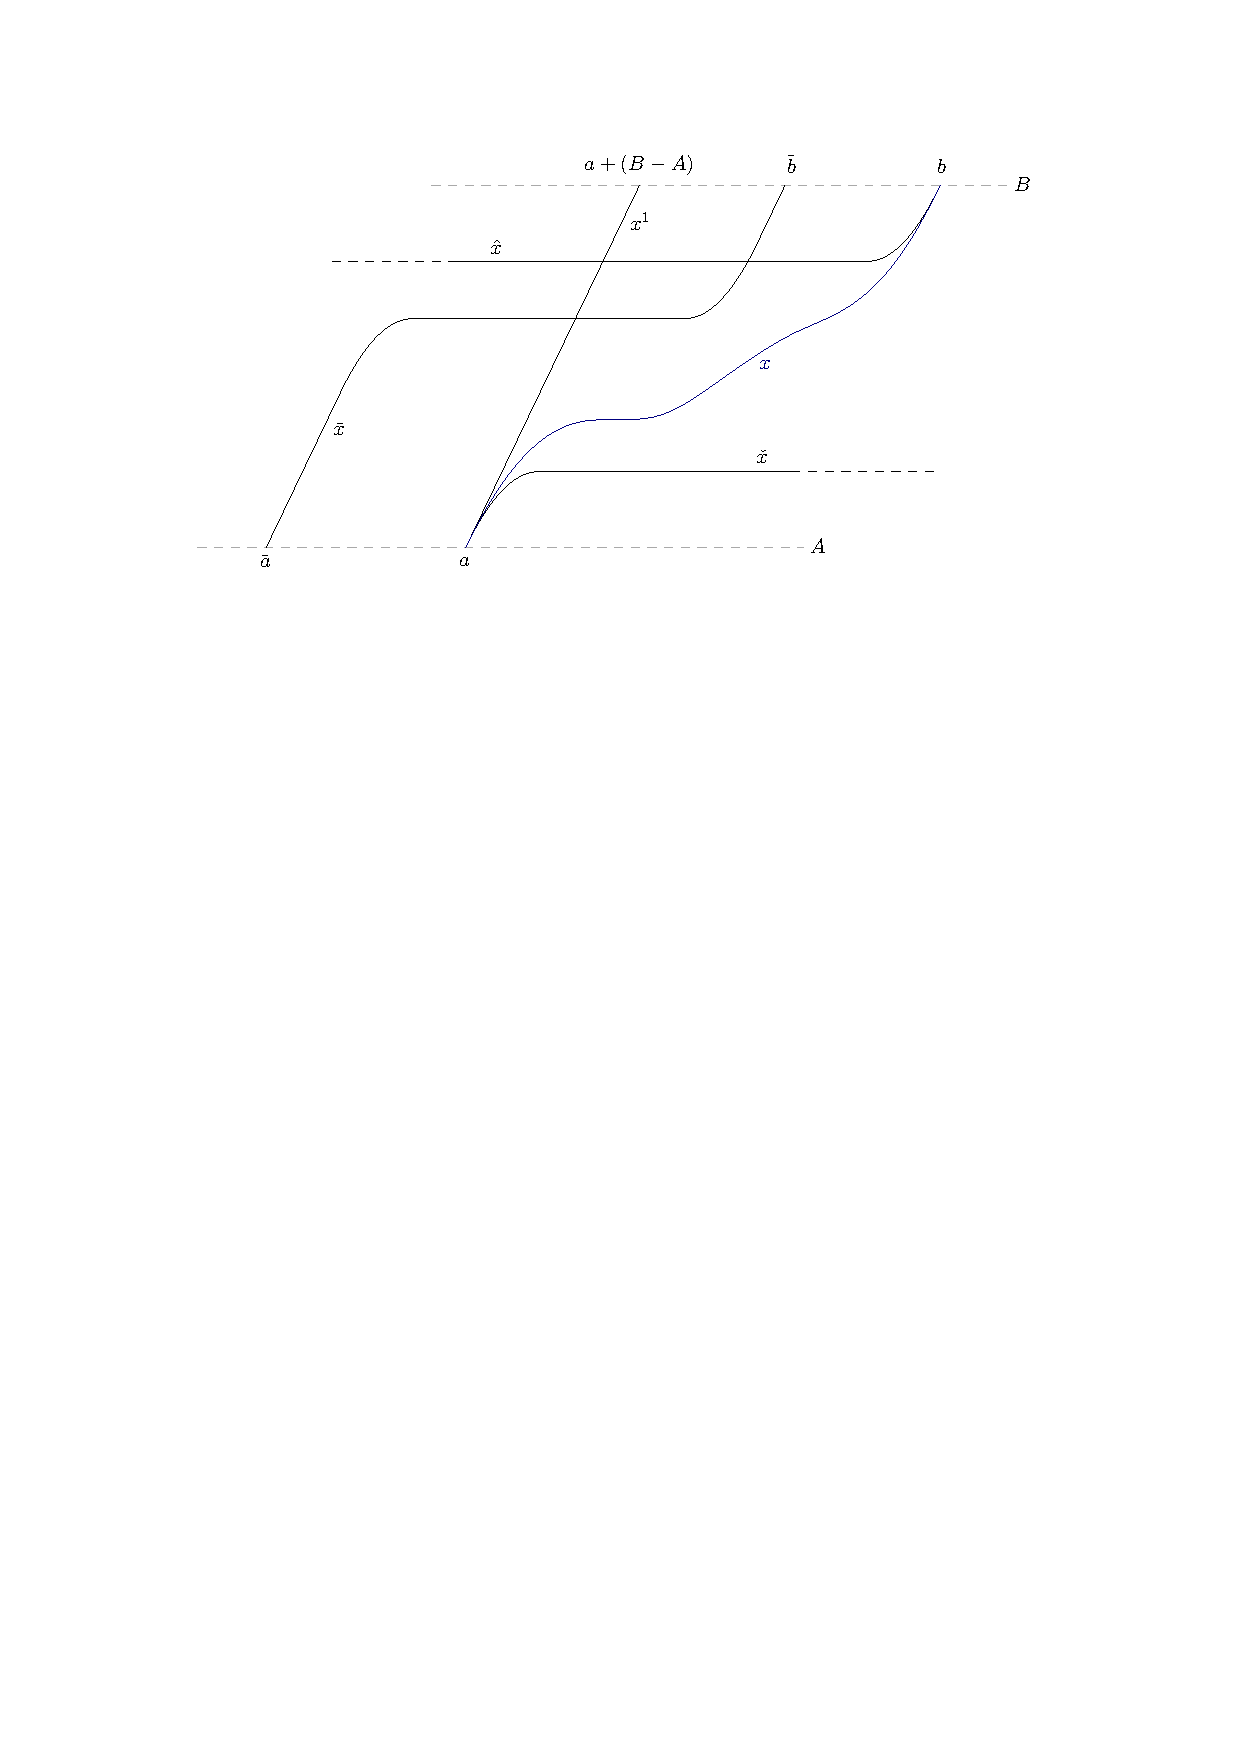
\includegraphics[scale=0.9]{figures/motion/necessary-conditions}
  \caption{Illustration of the four bounding trajectories
    $u, x^{1}, \hat{x}, \check{x}$ that bound feasible trajectories from
    above and below. We also drew an example of a feasible trajectory $x$ in
    blue. The horizontal axis represents time and the vertical axis corresponds
    to the position on the lane, so the vertical dashed grey lines correspond to
    the start and end of the lane.}%
  \label{fig:necessary-conditions}
\end{figure}

\begin{lemma}\label{lemma:necessary-conditions}
  Consider some lead vehicle constraint $u \in D_{1}[c,d]$ and assume there
  exists a trajectory $x \in D_{2}[a, b]$ such that $x \preceq u$, then the following
  conditions must hold \TabPositions{3cm}
  \begin{enumerate}[label=(\roman*)\quad,leftmargin=5em,midpenalty=5]
    \item $b-a \geq B-A$, \tab (full speed constraint)
    \item $d \leq b$, \tab (exit order constraint)
    \item $c \leq a$, \tab (entry order constraint)
    \item $u \succeq \check{x}$. \tab (entry space constraint)
  \end{enumerate}
\end{lemma}
\pagebreak[1]
\begin{proof}
  Each of these conditions corresponds somehow to one of the four bounding
  trajectories defined above.
  %
  Observe that $x^{1}(s) = B$ for $s = a + (B-A)$, which can be interpreted as
  the earliest time of departure from the lane. This shows that
  $b \geq a + (B-A)$, which is equivalent with (i).
  %
  % When (i) is violated, $x$ must cross $x^{1}$ somewhere, which means that the
  % maximum speed constraint must be violated.
  When either (ii) or (iii) is violated, the constraint $x \preceq u$ conflicts
  with one of the boundary conditions $x(a) = A$ or $x(b) = B$. To see that (iv)
  must hold, suppose that $u(\tau) < \check{x}(\tau)$ for some time $\tau$. Since
  $c \leq a$, this means that $u$ must intersect $\check{a}$ from above. Therefore,
  any trajectory that satisfies $x \preceq u$ must also intersect $\check{a}$
  from above, which contradicts the assumption $x \in D_{2}[a,b]$.
\end{proof}

We note that the boundaries $\hat{x}$ and $\check{x}$ can be combined to
yield yet another necessary condition.
%
It is straightforward to verify from~\cref{eq:hat-x,eq:check-x} that
$\hat{x}(t) \geq B - 1/(2\bar{\omega})$ and $\check{x}(t) \leq A + 1/(2\omega)$.
%
Therefore, whenever $B - A < 1/(2\bar{\omega}) + 1/(2\omega)$, these boundaries intersect
for certain values of $a$ and $b$.
%
Because the exact condition is somewhat cumbersome to characterize, we avoid
this case by simply assuming that the lane length is sufficiently large, to keep
the analysis simpler.

\begin{assump}\label{assump:lane-length}
  The length of the lane satisfies $B - A \geq 1/(2\omega) + 1/(2\bar{\omega})$.
\end{assump}

\noindent
Observe that $1/(2\omega)$ is precisely the distance required to decelerate from
full speed to a standstill. Similarly, $1/(2\bar{\omega})$ is the distance
required for a full acceleration. Therefore, we may interpret
Assumption~\ref{assump:lane-length} as requiring enough space in the lane such
that there is at least one \emph{waiting position}.
%
We will return to this observation in
Section~\ref{sec:feasibility-inequalities}.
\note{(check that we do this)}


\subsection{Constructing smooth upper boundary}\label{sec:optimal-trajectory}

\begin{figure}
  \centering
  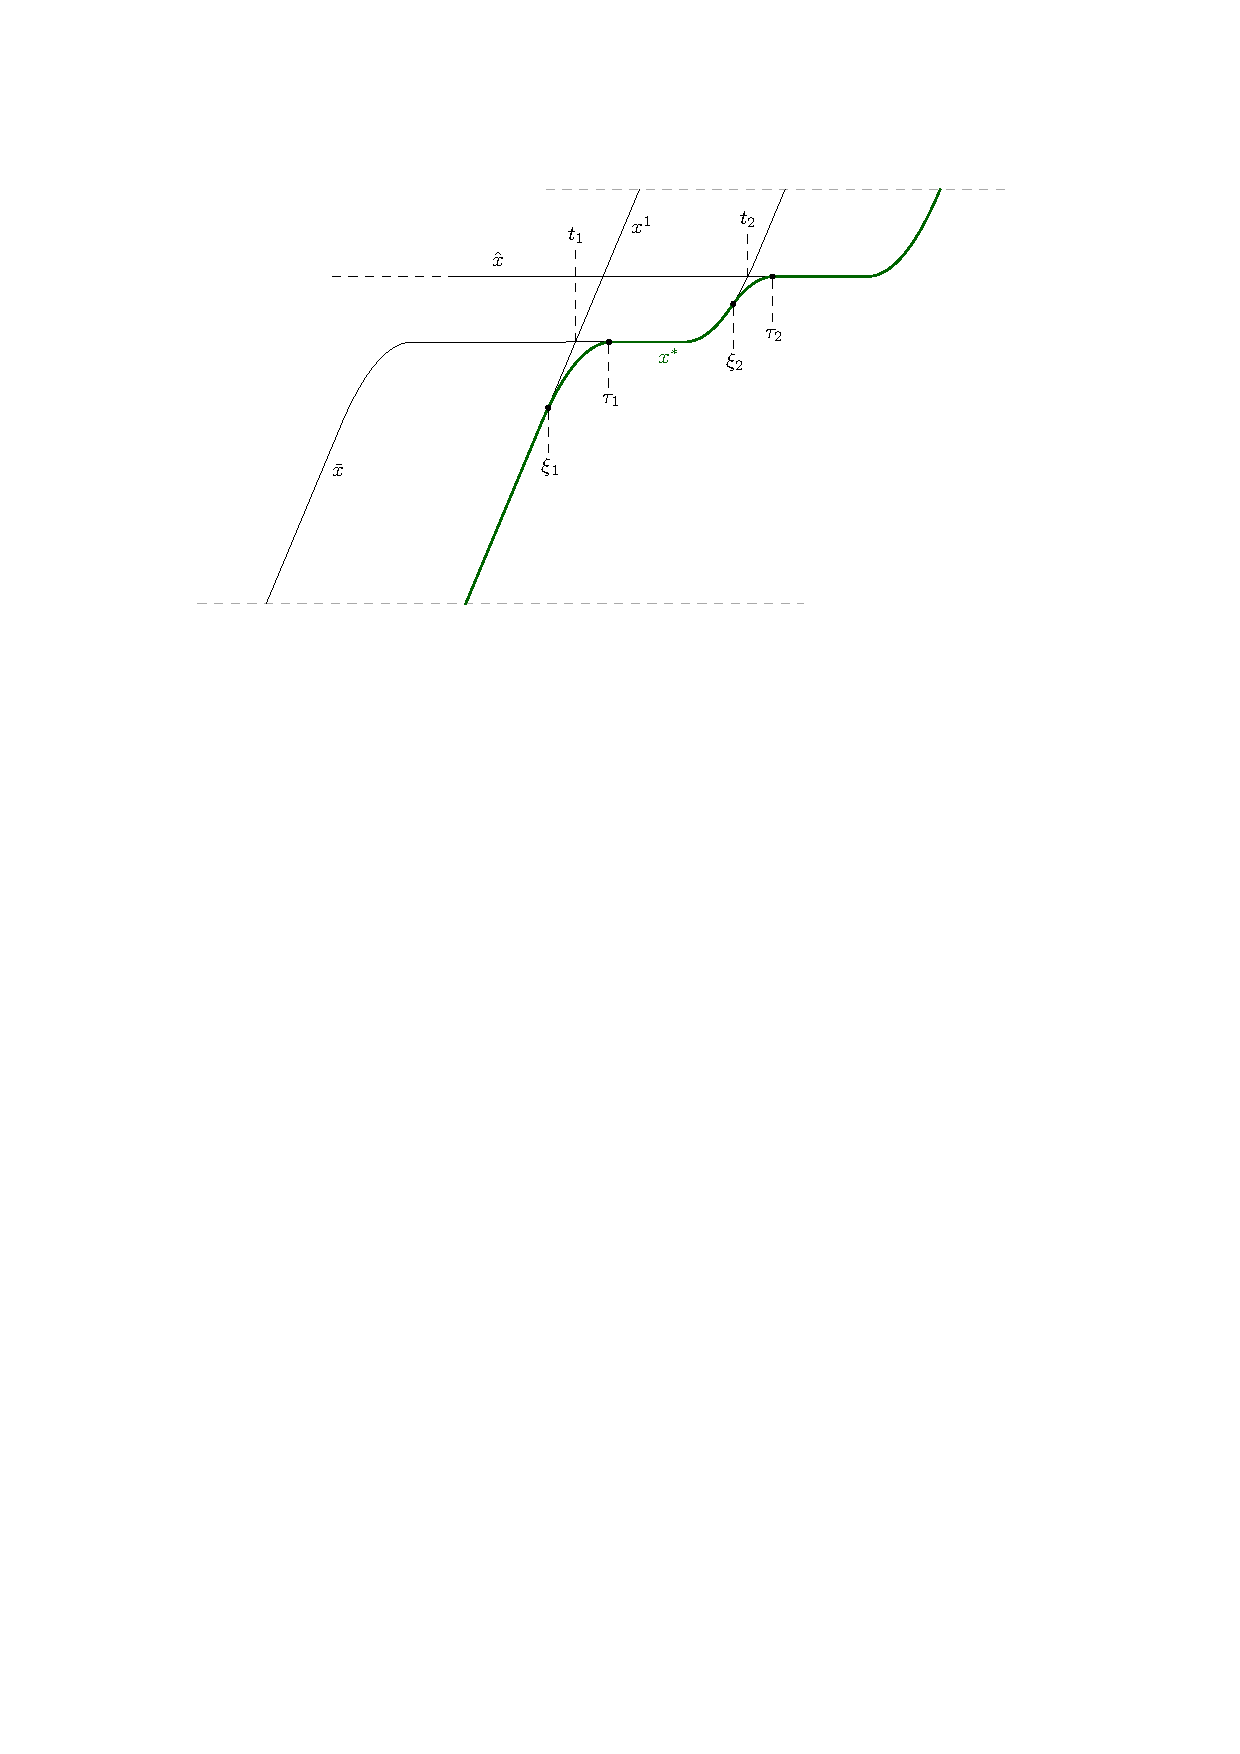
\includegraphics[scale=1]{figures/motion/proof}
  \caption{The minimum boundary $\gamma$, induced by three upper boundaries
    $u$, $\hat{x}$ and $x^{1}$, is smoothened around time $t_{1}$ and
    $t_{2}$, where the derivative is discontinuous, to obtain the smooth optimal
    trajectory $x^{*}$, drawn in green. The times $\xi_{i}$ and $\tau_{i}$
    correspond to the start and end of the connecting deceleration as
    defined in Section~\ref{sec:smoothing}.}%
  \label{fig:optimal-construction}
\end{figure}

Assuming the four conditions of Lemma~\ref{lemma:necessary-conditions} hold, we will show that we can always
construct a solution $\gamma^{*}$ for the single vehicle problem, thereby
showing that the four conditions are also sufficient.
%
The particular solution that we will construct is a smooth upper boundary for all
other solutions, in the sense that, for any other feasible solution $x$ we have
$x \preceq \gamma^{*}$.
%
The starting point is the \emph{minimum boundary} $\gamma : [a,b] \rightarrow \mathbb{R}$, defined as
\begin{align}\label{eq:min-boundary}
  \gamma(t) := \min \{ u(t), \hat{x}(t), x^{1}(t) \} .
\end{align}
%
Obviously, $\gamma$ is a valid upper boundary for any other feasible solution,
%
but in general, $\gamma$ may have a discontinuous derivative at some\footnote{In fact, it can be shown that, under the necessary conditions, there are at most two of such discontinuities.} isolated
points in time, in which case $\gamma \notin \mathcal{D}[a,b]$.

\begin{define}\label{def:piecewise-trajectory}
  Let $\mathcal{P}[a,b]$ be the set of functions $\mu : [a, b] \rightarrow \mathbb{R}$ for
  which there is a finite subdivision $a = t_{0} < \cdots < t_{n+1} = b$ such that
  the truncation $\mu|_{[t_{i}, t_{i+1}]} \in \mathcal{D}[t_{i}, t_{i+1}]$ is
  a smooth trajectory, for each $i \in \{0, \dots, n\}$, and for which the one-sided limits of $\dot{\mu}$ satisfy
  \begin{align}
    \dot{\mu}(t_{i}^{-}) := \lim_{t \uparrow t_{i}} \dot{\mu}(t) > \lim_{t \downarrow t_{i}} \dot{\mu}(t) =: \dot{\mu}(t_{i}^{+}) ,
  \end{align}
  for each $i \in \{1, \dots, n\}$. We refer to such $\mu$ as a \emph{piecewise
    trajectory (with downward bends)}.
\end{define}

It is not difficult to see from Figure~\ref{fig:necessary-conditions} that,
under the necessary conditions, $\gamma$ satisfies the above definition, so
$\gamma \in \mathcal{P}[a,b]$. In other words, $\gamma$ consists of a number of
pieces that are smooth and satisfy the vehicle dynamics, with possibly some
sharp bend downwards where these pieces come together.
%
Next, we present a simple procedure to smoothen out this kind of discontinuity
by decelerating from the original trajectory somewhat before some $t_{i}$, as
illustrated in Figure~\ref{fig:optimal-construction}. We will argue that this procedure can be repeated as
many times as necessary to smoothen out every discontinuity.


In Section~\ref{sec:deceleration-boundary}, we first define a parameterized
family of functions to model the deceleration part that we introduce for the
smoothing procedure, which is described in Section~\ref{sec:smoothing}.
%
We apply this procedure to $\gamma$ to obtain $\gamma^{*}$, after which it is
relatively straightforward to show that $\gamma^{*}$ is an upper bound for all
other feasible solutions, which is done in
Section~\ref{sec:upper-bound-property}


\subsubsection{Deceleration boundary}\label{sec:deceleration-boundary}
% In order to formalize the smoothing procedure, we will first define some
% parameterized family of functions to model the deceleration part that we
% introduce to smooth the original trajectory.
%
Recall the derivation of $\check{x}$ in equation~\eqref{eq:check-x} and the discussion
preceding it, which we will now generalize a bit.
%
Let $x \in \mathcal{D}[a, b]$ be some smooth trajectory, then observe that $\dot{x}(t) \geq \dot{x}(\xi) - \omega(t - \xi)$ for all $t \in [a, b]$.
Combining this with the constraint $\dot{x}(t) \in [0, 1]$, this yields
\begin{align}
  \dot{x}(t) \geq \max\{ 0, \, \min\{1, \, \dot{x}(\xi) - \omega (t - \xi) \}\} =: \{\dot{x}(\xi) - \omega(t-\xi)\}_{[0,1]} ,
\end{align}
where use $\{ \cdot \}_{[0,1]}$ as a shorthand for this clipping operation.
%
Hence, for any $t \in [a,b]$, we obtain the following lower bound
\begin{align}\label{eq:deceleration-boundary}
  x(t) = x(\xi) + \int_{\xi}^{t} \dot{x}(\tau) \diff \tau \geq x(\xi) + \int_{\xi}^{t} \{\dot{x}(\xi) - \omega(\tau - \xi)\}_{[0,1]} \diff \tau =: x[\xi] (t) ,
\end{align}
where we will refer to the right-hand side as the \emph{deceleration boundary} of $x$
at $\xi$.
%
Observe that this definition indeed generalizes the definition of $\check{x}$,
because we have $\check{x}=(x[a])|_{[a,b]}$.

Note that $x[\xi]$ depends on $x$ only through the two real numbers $x(\xi)$ and
$\dot{x}(\xi)$. It will be convenient later to rewrite the right-hand side
of~\eqref{eq:deceleration-boundary} as
\begin{align}\label{eq:def-x-}
  x^{-}[p, v, \xi](t) := p + \int_{\xi}^{t} \{ v - \omega(\tau - \xi) \}_{[0,1]} \diff \tau ,
\end{align}
such that $x[\xi](t) = x^{-}[x(\xi), \dot{x}(\xi), \xi](t)$.
%
We can expand the integral in this expression further by carefully handling the
clipping operation. Observe that the expression within the clipping operation
reaches the bounds $1$ and $0$ for $\delta_{1} := \xi - (1-v)/\omega$ and
$\delta_{0} := \xi + v/\omega$, respectively. Using this notation, a straightforward
calculation shows that
\begin{align}\label{eq:x-}
  x^{-}[p,v,\xi](t) = p +
  \begin{cases}
    {(1 - v)}^{2} / (2\omega) + (t - \xi) & \text{ for } t \leq \delta_{1} , \\
    v(t - \xi) - \omega{(t-\xi)}^{2} /2 & \text{ for } t \in [\delta_{1} , \delta_{0}] , \\
    v^{2}/(2\omega) & \text{ for } t \geq \delta_{0} .
  \end{cases}
\end{align}
%
It is easily verified that the three cases above coincide at
$t \in \{\delta_{1}, \delta_{0}\}$, which justifies the overlaps in the case distinction.
Furthermore, since $x$ and $\dot{x}$ are continuous by assumption, it follows
that $x[\xi](t) = x^{-}[x(\xi), \dot{x}(\xi), \xi](t)$ is continuous as a function of
either of its arguments.\footnote{Even more, it can be shown that $x[\xi](t)$ is continuous as a function of $(\xi, t)$.}
%
Assuming $0 \leq v \leq 1$, it can be verified that for every $t \in \mathbb{R}$, we
have $\ddot{x}^{-}[p,v,\xi](t) \in \{-\omega, 0\}$ and
$\dot{x}^{-}[p,v,\xi](t) \in [0,1]$ due to the clipping operation, so that
$x^{-}[p,v,\xi] \in \mathcal{D}(-\infty,\infty)$.

\begin{figure}
  \centering
  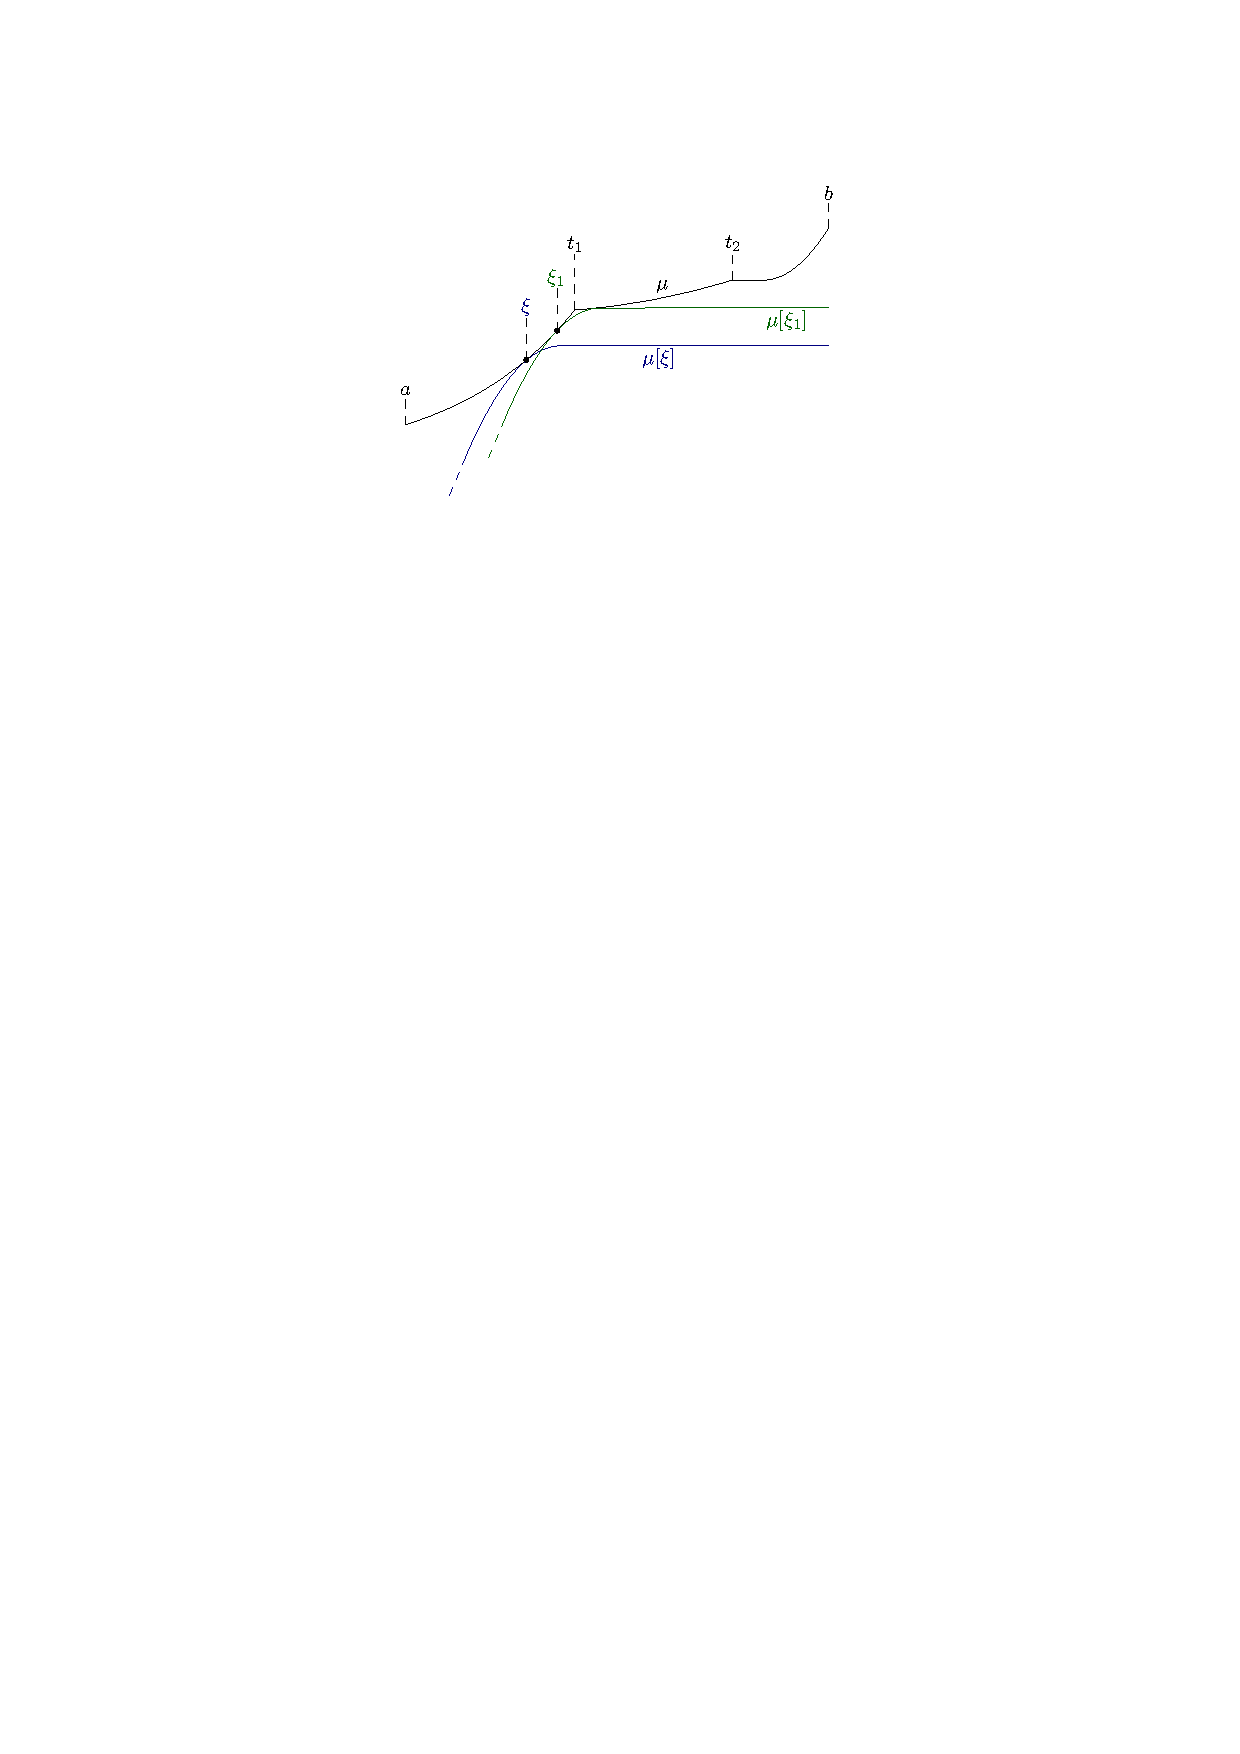
\includegraphics[scale=1.1]{figures/motion/deceleration-boundary}
  \caption{Illustration of some piecewise trajectory $\mu \in \mathcal{P}[a,b]$ with
    a discontinuous derivative at times $t_{1}$ and $t_{2}$. Furthermore, the
    figure shows some arbitrary deceleration boundary $\mu[\xi]$ at time $\xi$ in blue
    and the unique connecting deceleration $\mu[\xi_{1}]$ to the cover discontinuity at
    $t_{1}$ in green. We truncated the start of both deceleration boundaries for
    a more compact figure. The careful observer may notice that $\mu$ cannot occur
    as the minimum boundary defined in~\eqref{eq:min-boundary}, but please note that the class of
    piecewise trajectories $\mathcal{P}[a,b]$ is just slightly more general than
    necessary for our current purposes.}%
  \label{fig:deceleration-boundary}
\end{figure}


\paragraph{Piecewise trajectories.}
Let $\mu \in \mathcal{P}[a, b]$ be some piecewise trajectory with corresponding
subdivision $a = t_{0} < \cdots < t_{n+1} = b$ as defined in Definition~\ref{def:piecewise-trajectory}. It is
straightforward to generalize the definition of a deceleration boundary to $\mu$.
%
Whenever $\xi \in [a,b] \setminus \{ t_{1}, \dots, t_{n}\}$, we just define
$\mu[\xi] := x^{-}[\mu(\xi), \dot{\mu}(\xi), \xi]$, exactly like we did for $x$.
%
However, at the points of discontinuity $\xi \in \{ t_{1}, \dots, t_{n}\}$, the
derivative $\dot{\mu}(\xi)$ is not defined, so we choose to use the left-sided limit
instead, by defining $\mu[\xi] := x^{-}[\mu(\xi), \dot{\mu}(\xi^{-}), \xi]$.

\begin{remark}\label{rem:lower-bound-piecewise}
  Please note that we cannot just replace $x$ with $\mu$ in inequality~\eqref{eq:deceleration-boundary} to
  obtain a similar bound for $\mu$ on the its full interval $[a,b]$.
  Instead, we get the following \emph{piecewise lower bounding} property.
  %
  Consider some interval
  $I \in \{ [a, t_{1}], \openhalf{t_{1}}{t_{2}}, \dots, \openhalf{t_{n}}{b} \}$, then what
  remains true is that $\xi \in I$ implies $\mu(t) \geq \mu[\xi](t)$ for every $t \in I$.
\end{remark}


\subsubsection{Smoothing procedure}\label{sec:smoothing}
Let $\mu \in \mathcal{P}[a,b]$ be some piecewise trajectory and let
$a = t_{0} < \cdots < t_{n+1} = b$ denote the subdivision as in Definition~\ref{def:piecewise-trajectory}.
%
We first show how to smoothen the discontinuity at $t_{1}$ and then argue how to
repeat this process for the remaining times $t_{i}$.
Our aim is to choose some time $\xi \in [a,t_{1}]$ from which the vehicle starts
fully decelerating, such that $\mu[\xi] \preceq \mu$ and such that $\mu[\xi]$ touches $\mu$ at some time
$\tau \in [t_{1}, b]$ tangentially.
%
We will show there is a unique trajectory $\mu[\xi]$ that satisfies these requirements
and refer to it as the \emph{connecting deceleration}, see
Figure~\ref{fig:deceleration-boundary} for an example.
%
The construction relies on the following technical assumption.

\begin{assump}\label{assump:smoothing}
  Throughout the following discussion, we assume $\mu \succeq \mu[a]$ and $\mu \succeq \mu[b]$.
\end{assump}



\paragraph{Touching.}
Recall Remark~\ref{rem:lower-bound-piecewise}, which asserts that we have
$\mu[\xi](t) \leq \mu(t)$ for every $t \in [a,t_{1}]$ for any $\xi \in [a, t_{1}]$.
%
After the discontinuity, so for every $t \in [t_{1}, b]$, we want
$\mu[\xi](t) \leq \mu(t)$ and equality at least somewhere, so we measure the relative
position of $\mu[\xi]$ with respect to $\mu$ here, by considering
\begin{align}
  d(\xi) := \min_{t \in [t_{1}, b]} \mu(t) - \mu[\xi](t) .
\end{align}
Since $\mu(t)$ and $\mu[\xi](t)$ are both continuous as a function of $t$ on the interval
$[t_{1}, b]$, this minimum actually exists (extreme value theorem).
%
Furthermore, since $d$ is the minimum of a continuous function over a closed
interval, it is continuous as well (see Lemma~\ref{lemma:inf-continuous}).
%
Observe that $d(a) \geq 0$, because $\mu \succeq \mu[a]$ by Assumption~\ref{assump:smoothing}.
%
By definition of $t_{1}$, we have $\dot{\mu}(t_{1}^{-}) > \dot{\mu}(t_{1}^{+})$,
from which it follows that $\mu(t) < \mu[t_{1}](t)$ for $ t\in (t_{1}, t_{1} + \epsilon)$ for some
small $\epsilon > 0$, which shows that $d(t_{1}) < 0$.
%
By the intermediate value theorem, there is $\xi_{1} \in \halfopen{a}{t_{1}}$ such
that $d(\xi_{1}) = 0$.
%
This shows that $\mu[\xi_{1}]$ touches $\mu$ at some time
$\tau_{1} \in [t_{1}, b]$.


\paragraph{Uniqueness.}
It turns out that $\xi_{1}$ itself is not necessarily unique, which we explain
below. Instead, we are going to show that the connecting deceleration
$\mu[\xi_{1}]$ is unique. More precisely, given any other $\xi \in \halfopen{a}{t_{1}}$ such
that $d(\xi) = 0$, we will show that $\mu[\xi] = \mu[\xi_{1}]$.

The first step is to establish that the level set
\begin{align}
  X := \{ \xi \in \halfopen{a}{t_{1}} : d(\xi) = 0 \}
\end{align}
is a closed interval. To this end, we show that $d$ is non-increasing on
$\halfopen{a}{t_{1}}$, which together with continuity implies the desired result
(see Lemma~\ref{lemma:levelset}).
%
To show that $d$ is non-increasing, it suffices to show that $\mu[\xi](t)$ is
non-decreasing as a function of $\xi$, for every $t \in [t_{1}, b]$.
%
We can do this by computing the partial derivative of $\mu[\xi]$ with respect to $\xi$
and verifying it is non-negativity.
%
Recall the definition of $\mu[\xi]$, based on $x^{-}$ in equation~\eqref{eq:x-}.
%
Using similar notation, we write
$\delta_{1}(\xi) = \xi - (1 - \dot{\mu}(\xi))/\omega$ and
$\delta_{0}(\xi) = \xi + \dot{\mu}(\xi)/\omega$ and compute
%
\begin{align}
  \frac{\partial}{\partial \xi} \mu[\xi](t) =
  \dot{\mu}(\xi) +
  \begin{cases}
    \ddot{\mu}(\xi)(\dot{\mu}(\xi)-1)/\omega - 1 &\text{ for } t \leq \delta_{1}(\xi) , \\
    \ddot{\mu}(\xi)(t-\xi) - \dot{\mu}(\xi) + \omega(t-\xi) &\text{ for } t \in [\delta_{1}(\xi),\delta_{0}(\xi)] , \\
    \ddot{\mu}(\xi)\dot{\mu}(\xi)/ \omega &\text{ for } t \geq \delta_{0}(\xi) .
  \end{cases}
\end{align}
%
It is easily verified that the cases match at
$t \in \{\delta_{1}(\xi), \delta_{0}(\xi)\}$, which justifies the overlaps there.
%
Consider any $\xi \in \halfopen{a}{t_{1}}$ and $t \in [t_{1}, b]$, then we always have
$\delta_{1}(\xi) \leq \xi \leq t$, so we only have to verify the second and third case:
%
\begin{subequations}
\begin{alignat}{2}
  \frac{\partial}{\partial \xi} \mu[\xi](t) &= (\ddot{\mu}(\xi) + \omega)(t-\xi) \geq 0 \quad\quad\quad &&\text{ for } t \in [\delta_{1}(\xi) ,\delta_{0}(\xi)], \label{eq:case2} \\
  \frac{\partial}{\partial \xi} \mu[\xi](t) &\geq \dot{\mu}(\xi) + (-\omega)\dot{\mu}(\xi)/\omega = 0 &&\text{ for } t \geq \delta_{0}(\xi) . \label{eq:case3}
\end{alignat}
\end{subequations}
%
This concludes the argument for $X$ being a closed interval.

Assuming $\xi$ to be fixed, observe that there is equality in~\eqref{eq:case2} for some
$t \in [\delta_{1}(\xi), \delta_{0}(\xi)]$ if and only if there is equality in~\eqref{eq:case3}
for some other $t' \geq \delta_{0}(\xi)$. Note that this happens precisely when
$\ddot{\mu}(\xi) = -\omega$.
%
Therefore, whenever $\mu$ is fully deceleration, so $\dot{\mu}(t)=-\omega$ on
some open interval $U \subset (a, t_{1})$, we have
$(\partial/\partial \xi) \mu[\xi](t) = 0$ for all $t \geq \delta_{1}(\xi)$.
%
This essentially means that any choice of $\xi \in U$ produces the same
trajectory $\mu[\xi]$. Please see Figure~\ref{fig:deceleration-boundary-unique}
for an example of this case.
%
This observation is key to the remaining uniqueness argument.

\begin{figure}[h]
  \centering
  \vspace*{0.5em}
  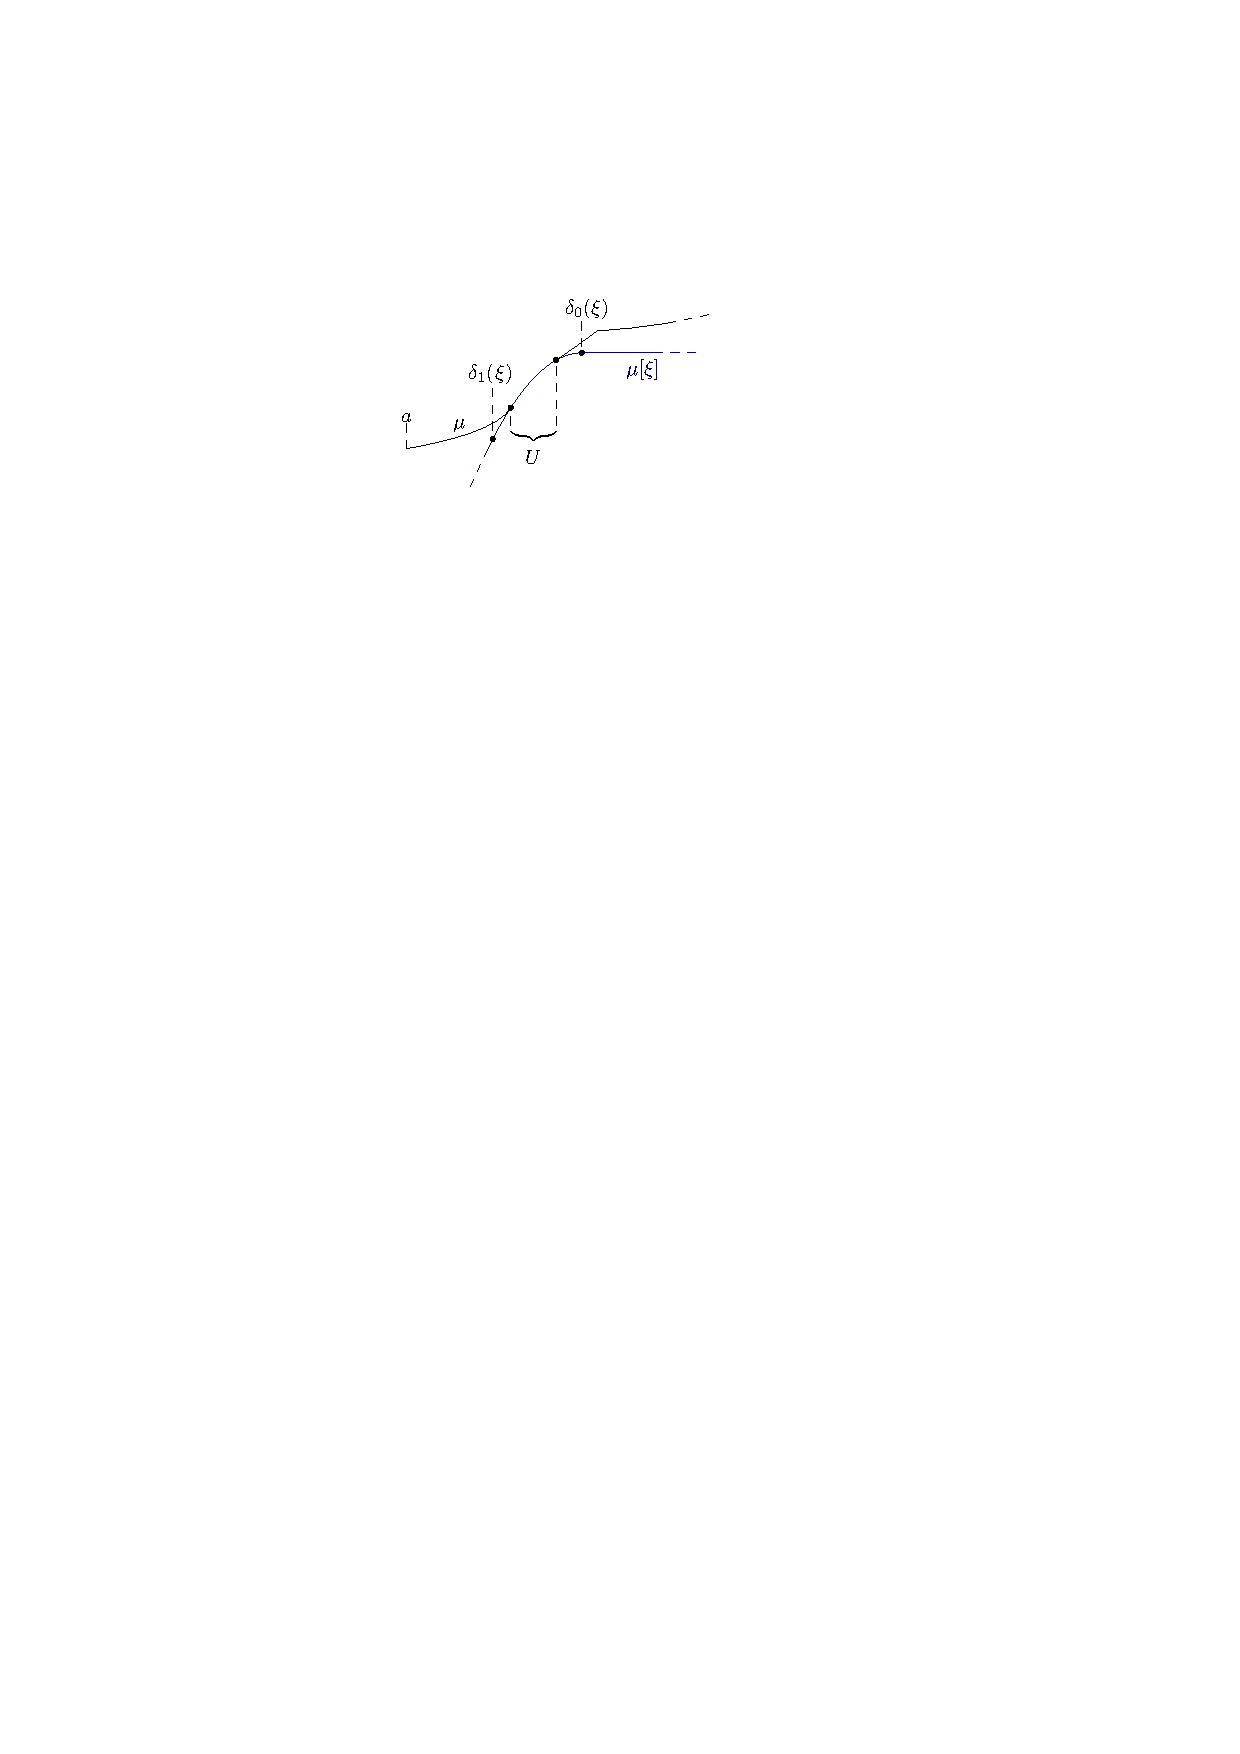
\includegraphics[scale=1.1]{figures/motion/deceleration-boundary-unique}
  \caption{Example of a piecewise trajectory $\mu$ with a part of full
    deceleration over some interval $U$ such that any choice of $\xi \in U$
    produces the same deceleration boundary $\mu[\xi]$, which naturally
    coincides with $\mu$ on $U$.}
  \label{fig:deceleration-boundary-unique}
\end{figure}

Since $X$ is a closed interval, we may define $\xi_{0} = \min X$.
%
Consider any $\xi' \in X$ with $\xi' > \xi_{0}$, then we show $\mu[\xi'](t) = \mu[\xi_{0}](t)$ for all
$t \in [\xi_{0}, b]$. For sake of contradiction, suppose there is some $t' \in [\xi_{0}, b]$ such that
$\mu[\xi'](t') > \mu[\xi_{0}](t')$, then there must be some open interval $U \subset (\xi_{0}, \xi')$ such that
\begin{align}\label{eq:positive-partial-derivative}
  \frac{\partial}{\partial \xi}\mu[\xi](t') > 0 \text{ for all } \xi \in U .
\end{align}
However, we argued in the previous paragraph that this actually holds for any
$t' \geq \delta_{1}(\xi)$.
%
In particular, let $t^{*} \in [t_{1}, b]$ be such that
$\mu(t^{*}) = \mu[\xi_{0}](t^{*})$, then
$t^{*} \geq t_{1} \geq \xi \geq \delta_{1}(\xi)$,
so~\eqref{eq:positive-partial-derivative} yields $\mu[\xi'](t^{*}) > \mu[\xi_{0}](t^{*})$, but then
$d(\xi') > d(\xi_{0}) = 0$, so $\xi' \notin X$, a contradiction.


\paragraph{Touching tangentially.}
\comment{I might add a figure for this whole part. Especially for the case tau1
  = b, because feasibility of the resulting trajectory relies on this.}
%
It remains to show that $\mu$ and $\mu[\xi_{0}]$ touch tangentially somewhere on
$[t_{1}, b]$. Let $\tau_{1} \in [t_{1}, b]$ be the smallest time such that
$\mu(\tau_{1}) - \mu[\xi_{0}](\tau_{1}) = d(\xi_{0}) = 0$ and consider the
following three cases.

First of all, note that $\tau_{1} = t_{1}$ is not possible, because this
would require
\begin{align}
  \dot{\mu}(t_{1}^{+}) > \dot{\mu}[\xi_{0}](t_{1}^{+}) = \dot{\mu}[\xi_{0}](t_{1}) ,
\end{align}
but since $\mu$ is a piecewise trajectory, we must have
$\dot{\mu}(t_{1}^{-}) > \dot{\mu}(t_{1}^{+}) > \dot{\mu}[\xi_{0}](t_{1})$. This
shows that $\mu(t_{1} - \epsilon) < \mu[\xi_{0}](t_{1} - \epsilon)$, for
some small $\epsilon > 0$, which contradicts $\mu[\xi_{0}] \preceq \mu$.

Suppose $\tau_{1} \in (t_{1}, b)$, then recall the definition of $d(\xi_{0})$
and observe that the usual first-order necessary condition (derivative zero) for
local minima requires $\dot{\mu}(\tau_{1}) = \dot{\mu}[\xi_{0}](\tau_{1})$.
\comment{I find this argument clear enough, but I am not sure if
  ''first-order necessary condition'', needs some further elaboration. It is
  just when you are minimizing some differentiable function f(x), then a local
  minimum a should have f'(a) = 0.}

Finally, consider $\tau_{1} = b$.
%
Observe that $\dot{\mu}(b) > \dot{\mu}[\xi_{0}](b)$, would contradict
minimality of $\tau_{1} = b$. Therefore, suppose
$\dot{\mu}(b) < \dot{\mu}[\xi_{0}](b)$, then
$\dot{\mu}[b](b) = \dot{\mu}(b) < \dot{\mu}[\xi_{0}](b)$, so
\begin{align}
  \dot{\mu}[b](t) \leq \dot{\mu}[\xi_{0}](t) \text{ for } t \leq b ,
\end{align}
but then $\mu[b](t) > \mu[\xi_{0}](t)$ for $t < b$. In particular, for $t=\xi_{0}$, this shows
$\mu[b](\xi_{0}) > \mu[\xi_{0}](\xi_{0}) = \mu(\xi_{0})$, which contradicts part $\mu[b] \preceq \mu$ of
Assumption~\ref{assump:smoothing}.


\paragraph{Repeat for remaining discontinuities.}
Let us summarize what we have established so far.
%
The times $\xi_{0} \in \halfopen{a}{t_{1}}$ and
$\tau_{1} \in \openhalf{t_{1}}{b}$ have been chosen such that
\begin{subequations}\label{eq:smoothing-requirements}
\begin{gather}
  \mu[\xi_{0}](t) \leq \mu(t) \; \text{ for } \; t \in [\xi_{0}, \tau_{1}] , \\
  \dot{\mu}[\xi_{0}](\xi_{0}) = \dot{\mu}(\xi_{0}) \; \text{ and } \; \dot{\mu}[\xi_{0}](\tau_{1}) = \dot{\mu}(\tau_{1}) .
\end{gather}
\end{subequations}
Instead of $\xi_{0}$, it will be convenient later to choose $\xi_{1} := \max X$
as the representative of the unique connecting deceleration.
%
We can now use $(\mu[\xi_{1}])|_{[\xi_{1},\tau_{1}]}$ to replace $\mu$ at $[\xi_{1}, \tau_{1}]$ to
obtain a trajectory without the discontinuity at $t_{1}$. More precisely, we
define
\begin{align}
  \mu_{1}(t) =
  \begin{cases}
    \mu(t) &\text{ for } t \in [a, \xi_{1}] \cup [\tau_{1}, b] , \\
    \mu[\xi_{1}](t) &\text{ for } t \in [\xi_{1}, \tau_{1}] .
  \end{cases}
\end{align}
From the way we constructed $\mu[\xi_{1}]$, it follows
from~\eqref{eq:smoothing-requirements} that we have
$\mu_{1} \in \mathcal{P}[a,b]$, but without the discontinuity at $t_{1}$.
%
Observe that a single connecting deceleration may cover more than one
discontinuity, as illustrated in Figure~\ref{fig:multiple-discontinuities}.
%
Note that we must have $\dot{\mu}_{1}(a) = \dot{\mu}(a)$ and
$\dot{\mu}_{1}(b) = \dot{\mu}(b)$ by construction.
%
Hence, it is not difficult to see that $\mu_{1}$ must still satisfy
Assumption~\ref{assump:smoothing}, so that we can keep repeating the exact same
process, obtaining connecting decelerations $(\xi_{2}, \tau_2), (\xi_{3}, \tau_{3}), \,\dots$
and the corresponding piecewise trajectories $\mu_{2}, \mu_{3}, \,\dots$ to remove any
remaining discontinuities until we end up with a smooth trajectory
$\mu^{*} \in \mathcal{D}[a,b]$.
%
We emphasize again that $\dot{\mu}^{*}(a) = \dot{\mu}(a)$ and
$\dot{\mu}^{*}(b) = \dot{\mu}(b)$.

\begin{figure}
  \centering
  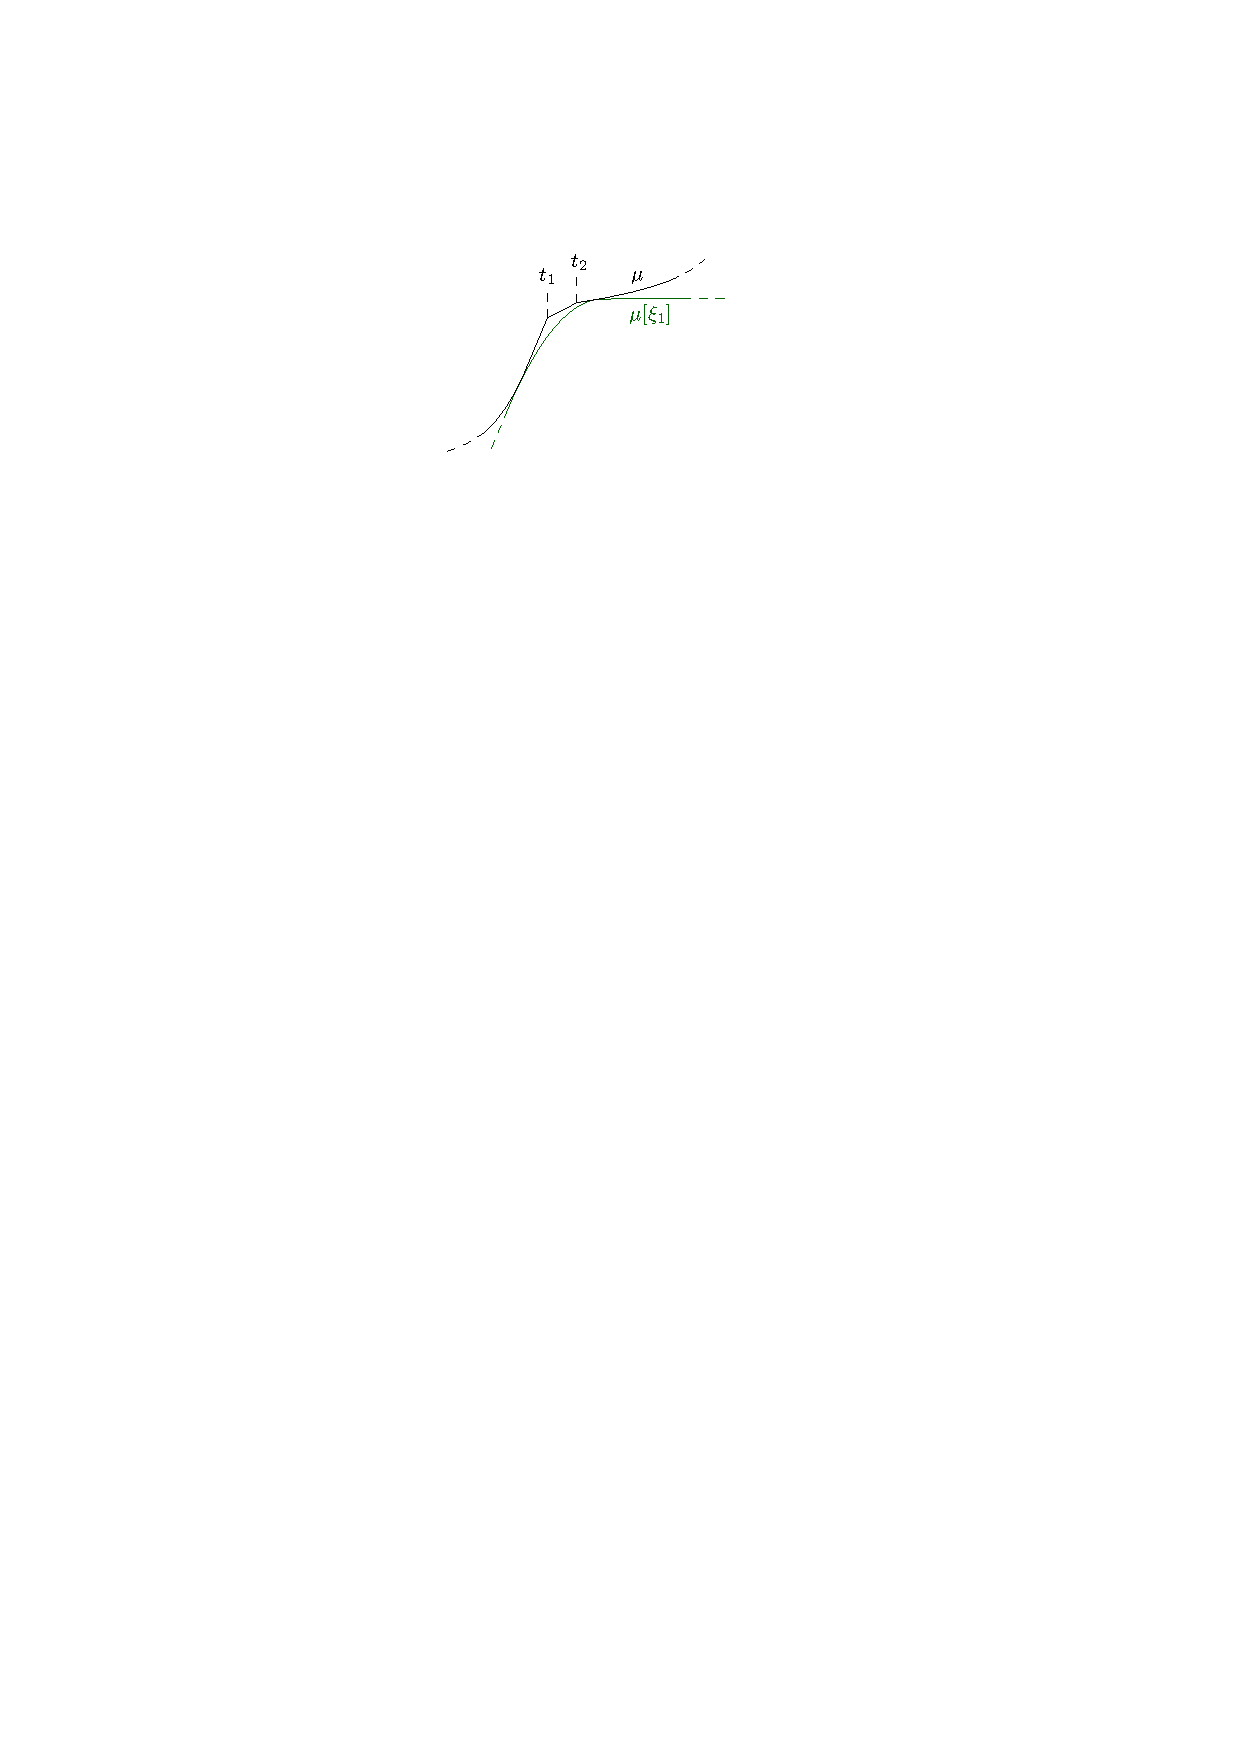
\includegraphics[scale=1.0]{figures/motion/multiple-discontinuities}
  \caption{Part of a piecewise trajectory $\mu$ on which a single connecting
    deceleration covers the two discontinuities at $t_{1}$ and $t_{2}$ at
    once.}%
  \label{fig:multiple-discontinuities}
\end{figure}


\subsubsection{Smooth upper boundary}\label{sec:upper-bound-property}

Let us now return to the minimum boundary $\gamma$ defined
in~\eqref{eq:min-boundary}.
%
From Figure~\ref{fig:necessary-conditions} and the necessary conditions, it is clear that $\gamma$ must satisfy
$\gamma(a) = A$, $\gamma(b) = B$ and \comment{I think this could be made more rigorous,
  but I think this is clear enough from the figure.}
$\dot{\gamma}(a) = \dot{\gamma}(b) = 1$, so whenever we have $\gamma \in \mathcal{D}[a, b]$,
i.e., $\gamma$ does not contain discontinuities, we automatically have
$\gamma \in D_{2}[a,b]$ so that $\gamma$ itself is already a feasible solution.
%
Otherwise, we perform the smoothing procedure presented above to obtain the
smoothed trajectory $\gamma^{*} \in \mathcal{D}[a,b]$.
%
The next lemma shows that $\gamma^{*}$ is an upper boundary for any feasible
trajectory.

\begin{lemma}\label{lemma:upperbound}
  Let $\mu \in \mathcal{P}[a,b]$ be a piecewise trajectory and let
  $\mu^{*} \in \mathcal{D}[a,b]$ denote the result after smoothing. All
  trajectories $x \in \mathcal{D}[a, b]$ that are such that
  $x \preceq \mu$, must satisfy $x \preceq \mu^{*}$.
  \comment{Is this argument clear enough?}
\end{lemma}
\begin{proof}
  Consider some interval $(\xi, \tau)$ where we introduced some connecting
  deceleration boundary. Suppose there exists some $t_{d} \in (\xi, \tau)$ such that
  $x(t_{d}) > \mu(t_{d})$. Because $x(\xi) \leq \mu(\xi)$, this means that $x$ must
  intersect $\mu$ at least once in $\halfopen{\xi}{t_{d}}$, so let
  $t_{c} := \sup \, \{ t \in \halfopen{\xi}{t_{d}} : x(t) = \mu(t) \}$ be the latest
  time of intersection such that $x(t) \geq \mu(t)$ for all $t \in [t_{c}, t_{d}]$.
  There must be some $t_{v} \in [t_{c}, t_{d}]$ such that $\dot{x}(t_{v}) > \dot{\mu}(t_{v})$,
  otherwise
  \begin{align*}
    x(t_{d}) = x(t_{c}) + \int_{t_{c}}^{t_{d}} \dot{x}(t) \diff t \leq \mu(t_{c}) + \int_{t_{c}}^{t_{d}} \dot{\mu}(t) \diff t = \mu(d_{t}) ,
  \end{align*}
  which contradicts our choice of $t_{d}$. Hence, for every
  $t \in [t_{v}, \tau]$, we have
  \begin{align*}
    \dot{x}(t) \geq \dot{x}(t_{v}) - \omega (t - t_{v}) > \dot{\mu}(t_{v}) - \omega(t - t_{v}) = \dot{\mu}(t) .
  \end{align*}
  It follows that $x(\tau) > \mu(\tau)$, which contradicts the assumption
  $x \preceq \mu$.
\end{proof}

\begin{remark}
  Observe that it follows from the above lemma that
  \begin{align}
    \int_{a}^{b} x(t) \diff t \leq \int_{a}^{b} \gamma^{*}(t) \diff t
  \end{align}
  for any other $x \in D_{2}[a,b]$ satisfying $x \preceq u$. Recall the haste
  criterion $J(x)$ defined in~\eqref{eq:haste-objective}, then we see that
  $\gamma^{*}$ is the optimal solution to the single vehicle optimal control
  problem
  \begin{align}
    \max_{x \in D_{2}[a,b]} J(x) \; \text{ such that } \; x \preceq u .
  \end{align}

\end{remark}

\newpage
\note{We will need this later\dots}

\paragraph{Acceleration boundary.}
Before we present the decomposition, we first define an auxiliary upper
boundary.
%
Similar to how we generalized the entry boundary $\check{x}$ to the deceleration
boundary in Section~\ref{sec:deceleration-boundary}, we now generalize the exit
boundary $\hat{x}$ to obtain the \emph{acceleration boundary}.
%
Because the derivation is completely analogous, we will only present the
resulting expressions.
%
Let $x \in \mathcal{D}[a,b]$ be some smooth trajectory, then the acceleration
boundary $x^{+}[\xi]$ of $x$ at some $\xi \in [a,b]$ is defined as the
right-hand side of the inequality
\begin{align}
  x(t) \leq x(\xi) + \int_{\xi}^{t} \{\dot{x}(\xi) + \bar{\omega} (\tau - \xi) \}_{[0,1]} \diff \tau =: x^{+}[\xi](t) ,
\end{align}
which holds for every $t \in [a,b]$.
%
Observe that the exit boundary can now be written as the restricted acceleration
boundary $\hat{x} = (x^{+}[b])|_{[a,b]}$.
%
Similar to definition~\eqref{eq:def-x-}, we define
\begin{align}
  x^{+}[p,v,\xi](t) := p + \int_{\xi}^{t}\{ v + \bar{\omega}(\tau - \xi)\}_{[0,1]} \diff \tau ,
\end{align}
such that $x^{+}[\xi](t) = x^{+}[x(\xi),\dot{x}(\xi),\xi](t)$ and
%
similar to~\eqref{eq:x-}, we calculate
\begin{align}
  x^{+}[p,v,\xi](t) = p +
  \begin{cases}
    \dots &\text{ for } t \leq \bar{\delta}_{0} , \\
    \dots &\text{ for } t \in [\bar{\delta}_{0}, \bar{\delta}_{1} ] , \\
    \dots &\text{ for } t \geq \bar{\delta}_{1} ,
  \end{cases}
\end{align}
with $\bar{\delta}_{0} := $ and $\bar{\delta}_{1} := $.

\newpage
\section{Lane planning feasibility}\label{sec:lane-problem-feasibility}

We will now return to the feasibility of the lane planning problem and show how
it decomposes in terms of a sequence of single vehicle feasibility problems.
%
\note{rewrite: We will see how the $x_{i}$ to each subproblem determines the
boundary $\bar{x}_{i+1}$ for the next subproblem.}
%
Moreover, we will state the feasibility of the lane planning problem in terms of
feasibility of the individual single vehicle problems, which will result in a
system of inequalities in terms of the schedule time vectors
$a = (a_{1}, \dots, a_{N})$ and $b = (b_{1}, \dots, b_{N})$.

\begin{assump}\label{assump:L-bound}
  Assume that $L < B - A$.
\end{assump}

\begin{lemma}\label{lemma:boundary-extension}
  Consider some trajectory $u \in \mathcal{D}[c,d]$ such that $u(d) \geq A$. If
  $x \in \mathcal{D}[a,b]$ is such that $x(a) = A$ and $x \preceq u$, then it
  satisfies $x \preceq (u(d) + t - d)|_{\halfopen{d}{\infty}}$, which may be
  interpreted as extending the upper boundary $u$ to the right at full speed.
\end{lemma}
\begin{proof}
  If $b < d$, then $x \preceq (\cdot)|_{\halfopen{d}{\infty}}$ is always void and
  the statement is trivially true. Assume $b \geq d$ and consider an arbitrary
  $t \geq d$.
  %
  Suppose $a \leq d$, then we have $x(t) \leq x(d) + t - d \leq u(d) + t - d$.
  Suppose $a > d$, then we have $x(t) \leq x(a) + t - a = A + t - a \leq u(d) + t - d$.
\end{proof}

For some $y \in \mathcal{D}[\alpha, \beta]$, we define the inverse at some position $p$ in
its range to be
\begin{align}
  y^{-1}(p) = \inf \{ t \in [\alpha, \beta] : y(t) = p\} .
\end{align}
%
Given some feasible trajectory $u \in D[c,d]$, we define its \emph{downshift}
%
\begin{align}
  \bar{u}(t) =
  \begin{cases}
    u(t) - L &\text{ for } t \in [u^{-1}(A + L), d] , \\
    B - L + t - d &\text{ for } t \in [d, d + L] .
  \end{cases}
\end{align}
For ease of reference, we denote the endpoints of its domain as
$\bar{a} := u^{-1}(A+L)$ and $\bar{b} := d + L$.

\begin{lemma}\label{lemma:downshift}
  For each $u \in D_{2}[c,d]$, the downshift trajectory satisfies
  $\bar{u} \in D_{1}[\bar{a},\bar{b}]$.
  %
  For each $x \in D[a, b]$ such that $a \geq c$ and $b \geq d$, we have
  $x \preceq u - L$ if and only if $x \preceq \bar{u}$.
\end{lemma}
\begin{proof}
  The two cases in the definition of $\bar{u}$ coincide, so that
  $\bar{u} \in \mathcal{D}$. Furthermore, it is easily verified that
  $\bar{u}(\bar{a}) = A$ and $\bar{u}(\bar{b}) = B$, so the first claim
  follows.

  Suppose $x \preceq u - L$, and suppose there exists some
  $t \in [a,b] \cap [c,d]$. If $t \in [\bar{a}, d]$, then
  $x(t) \leq u(t) - L = \bar{u}(t)$ by definition. If $t \in [d, \bar{b}]$, then
  apply Lemma~\ref{lemma:boundary-extension} to $u - L$ (using
  Assumption~\ref{assump:L-bound} for $u(d) - L \geq A$) to obtain
  $x \leq (\tau \mapsto u(d) - L + \tau - d)|_{\halfopen{d}{\infty}} = (\tau \mapsto B - L + \tau - d)|_{\halfopen{d}{\infty}}$,
  so that $x(t) \leq B - L + t - d = \bar{u}(t)$.

  For the other direction, suppose $x \preceq \bar{u}$. First of all, since
  $u(c) = A$ and $u(\bar{a}) = A+L > A$ and $u$ is non-decreasing, we have
  $c < \bar{a}$.
  %
  Suppose $c \leq a < \bar{a}$, then since $b \geq d \geq \bar{a}$ and
  $\dot{x}(a) = 1$, we must have
  $x(\bar{a}) > x(a) = A = \bar{u}(\bar{a})$, contradicting the initial
  assumption.
  %
  Hence, $a \geq \bar{a}$, so any $t \in [a,b] \cap [c,d]$ satisfies
  $t \in [u^{-1}(A+L), d]$, but then $x(t) \leq \bar{u}(t) = u(t) - L$ by
  definition.
\end{proof}


For brevity, we will write $x \in D_{2}^{N}[a, b]$ to denote the vector $x = (x_{1}, \dots, x_{N})$
of $N$ trajectories $x_{i} \in D_{2}[a_{i},b_{i}]$, while assuming that the
schedule times $a = (a_{1}, a_{2}, \dots, a_{N})$ and
$b = (b_{1}, b_{2}, \dots, b_{N})$ are ordered
$a_{1} \leq a_{2} \leq \dots \leq a_{N}$ and
$b_{1} \leq b_{2} \leq \dots \leq b_{N}$.

\begin{lemma}
  The following five statements are equivalent:

  \begin{enumerate}[leftmargin=3em]
    \item[(C0)] The lane planning problem is feasible.
    \item[(C1)] There exists $x \in D_{2}^{N}[a, b]$ such that $x_{i} \leq x_{i-1} - L$ for all $i \in \{2, \dots, N\}$.
    \item[(C2)] There exists $x \in D_{2}^{N}[a, b]$ such that $x_{i} \leq \bar{x}_{i-1}$ for all $i \in \{2, \dots, N\}$.

    \item[(C3)] There exists $x \in D_{2}^{N}[a, b]$ such that
          $b_{i} - a_{i} \geq B - A$ for all $i \in \{1, \dots, N\}$; and
    \TabPositions{2cm}
    \begin{enumerate}[label=(\roman*)\quad,leftmargin=3em,midpenalty=10]
      \item $b_{i} \geq \bar{b}_{i-1}$, \tab (exit order constraint)
      \item $a_{i} \geq \bar{a}_{i-1}$, \tab (entry order constraint)
      \item $\bar{x}_{i} \geq \check{x}_{i}$. \tab (entry space constraint)
    \end{enumerate}

    \item[(C4)] We have $b_{i} - a_{i} \geq B-A$ for all $i \in \{1, \dots, N\}$; and
    \begin{enumerate}[leftmargin=4em,midpenalty=10]
      \item[(ii*)\quad] $b_{i} \geq b_{i-1} + L$,
      \item[(iii*)\quad] $a_{i} \geq a_{i-1} + L$,
    \end{enumerate}
    for all $i \in \{2, \dots, N\}$; and
    \begin{enumerate}[leftmargin=4em,midpenalty=10]
      \item[(c*)\quad] $a_{i} \geq a^{*}$, \tab (capacity constraint)
    \end{enumerate}
    for all $i \in \{n, \dots, N \}$.
  \end{enumerate}
\end{lemma}
\begin{proof}
  Of course, (C0) and (C1) are equivalent by definition. Note that ``(C1) $\iff$
  (C2)'' is handled by Lemma~\ref{lemma:downshift}.

  We show ``(C2) $\implies$ (C3)''.

  We show ``(C3) $\implies$ (C2)''.

  We show ``(C?) $\implies$ (C4)''.

  We show ``(C4) $\implies$ (C?)''.
\end{proof}

\note{Special treatment of first vehicle.}


\newpage
\subsection{Decomposition}

Let the optimal solution of the single vehicle problem be denoted by
\begin{align}
  x^{*}(\alpha, \beta, \bar{x}) := \argmax_{x \in D[\alpha,\beta]} \int_{\alpha}^{\beta} x(t) \quad \text{ such that  } x \leq \bar{x}
\end{align}
and let $F_{1}(\alpha, \beta, \bar{x})$ denote the corresponding objective value.
%
We now restate the lane planning problem here for easy reference.
%
Assuming the system parameters $(\omega, \bar{\omega},A,B,L)$ to be fixed, given
some vector of arrival times $a = (a_{1}, \dots, a_{N})$ and departure times
$b = (b_{1}, \dots, b_{N})$, the goal is to maximize
\begin{subequations}
\begin{alignat}{3}
  &F(a,b) := \; &\max        \quad  & \sum_{i=1}^{N} \int_{a_{i}}^{b_{i}} x_{i}(t) \diff t , \\
  &             &\text{s.t.} \quad
  & x_{i} \in D[a_{i},b_{i}] & \text{ for each } i \in \{1, \dots, N\} , \\
  &&& x_{i} \leq x_{i-1} - L & \text{ for each } i \in \{2, \dots, N\} . \label{eq:follow-constraint}
\end{alignat}
\end{subequations}

%
Now consider the safe following constraints~\eqref{eq:follow-constraint}.
%
We show how to model these by
defining a boundary $\bar{x}_{i} \in \bar{D}[\bar{a}_{i}, \bar{b}_{i}]$ for each
$i \in \{2, \dots, N\}$, such that the single vehicle problem can be applied.
%
It becomes clear from Figure~\ref{fig:solution} that inequality~\eqref{eq:follow-constraint} only applies on some
subinterval $I_{i} \subset [a_{i-1}, b_{i-1}]$.
%
More specifically, by defining the inverse function
\begin{align}
  x_{i}^{-1}(p) := \inf \{ t: x_{i}(t) = p \} ,
\end{align}
it is easily seen that $I_{i} = [x_{i-1}^{-1}(A+L), b_{i-1}]$.
%
However, since $\dot{x}_{i-1}(b_{i-1}) = 1$, we can extend \comment{Let's leave
  it like this for now. I think that it is not too difficult to see that this
  works by looking at the figure, so no need to introduce more notational
  burden.} the boundary until $b_{i-1} + L$ without any problems. More
precisely, we define $\bar{a}_{i} := x_{i-1}^{-1}(A+L)$ and
$\bar{b}_{i} := b_{i-1}+L$ such that the boundary
$\bar{x}_{i} \in \bar{D}[\bar{a}_{i},\bar{b}_{i}]$ is given by
\begin{align}\label{eq:follow-boundary}
  \bar{x}_{i} :=
  \begin{cases}
    x_{i-1}(t) - L &\text{ for } t \in [\bar{a}_{i}, b_{i-1}] , \\
    t - b_{i-1} + B - L  &\text{ for } t \in [b_{i-1}, \bar{b}_{i}] .
  \end{cases}
\end{align}


Now, it is clear that the optimal trajectories $x_{i}$ are recursively given
by
\begin{subequations}
\begin{align}
  x_{1} &= x^{*}(a_{1}, b_{1}, \varnothing) , \\
  x_{i} &= x^{*}(a_{i}, b_{i}, \bar{x}_{i})  ,  \quad \text{ for } i \geq 2 ,
\end{align}
\end{subequations}
%
where we use the notation $\bar{x}_{1} = \varnothing$ to denote that the single vehicle
problem for the first vehicle $i=1$ does not have an active boundary
constraint.\footnote{Alternatively, we could think about this as having some $\bar{x} \in \bar{D}[\bar{a},\bar{b}]$ with very small $\bar{a} \ll a$ and $\bar{b} \ll b$.}
%
The corresponding total objective for the lane planning problem is simply given
by
\begin{align}
  F(a, b) = F_{1}(a_{1}, b_{1}, \varnothing) + \sum_{i=2}^{N} F_{1}(a_{i}, b_{i}, \bar{x}_{i}) .
\end{align}

\begin{figure}
  \centering
  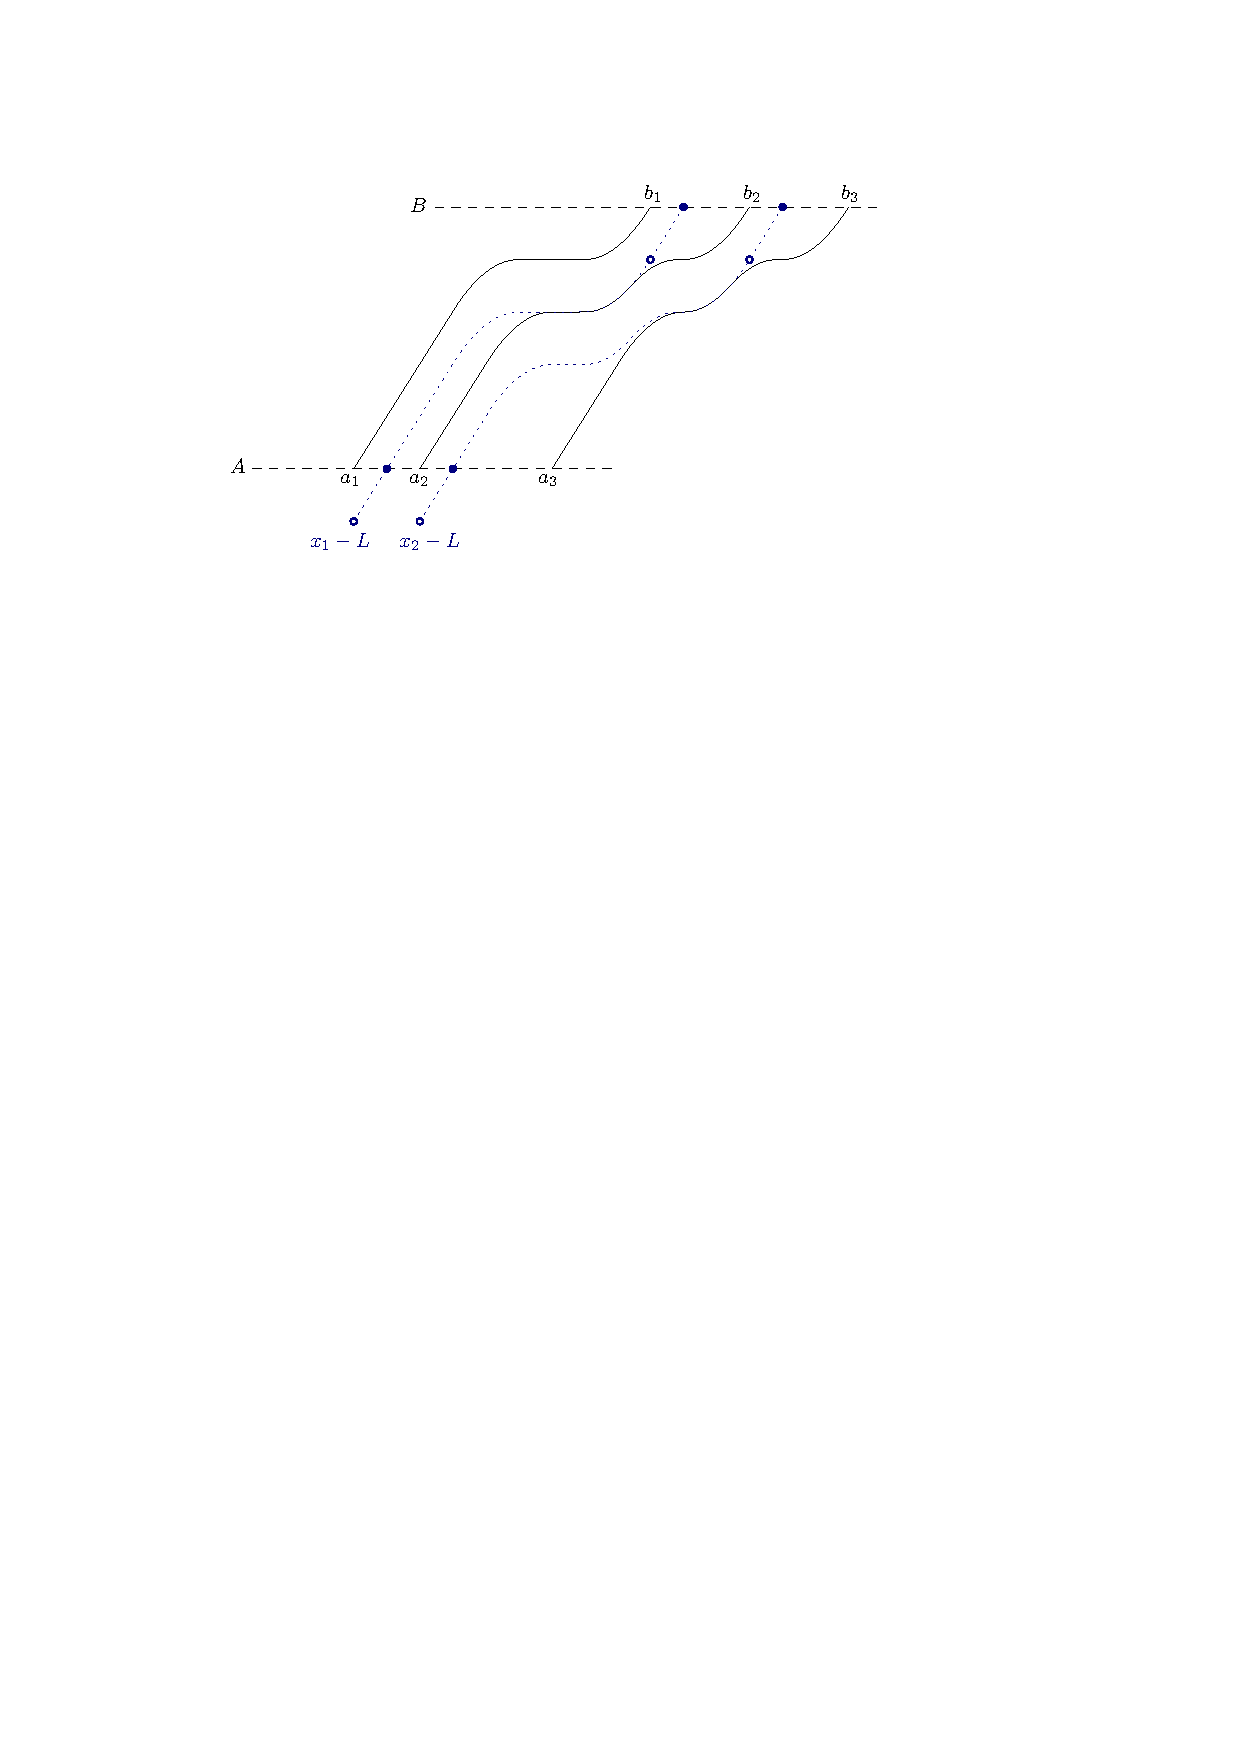
\includegraphics[scale=1.0]{figures/motion/solution}
  \caption{Optimal trajectories $x_{i}$ for three vehicles. The dotted blue
    trajectories between the little open circles illustrates the safe following
    constraints~\eqref{eq:follow-constraint}. The dotted blue trajectories between
    the solid dots are the following boundaries
    $\bar{x}_{2} \in \bar{D}[\bar{a}_{2}, \bar{b}_{2}]$ and
    $\bar{x}_{3} \in \bar{D}[\bar{a}_{3}, \bar{b}_{3}]$.}%
  \label{fig:solution}
\end{figure}

\newpage
\subsection{Feasibility as system of linear inequalities}\label{sec:feasibility-inequalities}

We showed above how to decompose the lane planning problem into
individual single vehicle problems by a simple construction of the boundary
$\bar{x}_{i}$, based on the trajectory $x_{i-1}$ of the preceding vehicle.
%
Recall Lemma~\ref{lemma:necessary-conditions}, which states the necessary
conditions for feasibility of the single vehicle problem. We showed in Section~\ref{sec:optimal-trajectory}
that these conditions are also sufficient.
%
We will restate them here for easy reference, applied to each single vehicle
problem belonging to the lane planning problem. By the construction at the
beginning of this section, it follows that the lane planning problem is feasible
if and only if each vehicle $i \in \{1, \dots, N\}$ satisfies the conditions:
%
\TabPositions{3cm}
\begin{enumerate}[label=(\roman*)\quad,leftmargin=5em,midpenalty=10]
  \item $b_{i}-a_{i} \geq B-A$, \tab (full speed constraint)
  \item $\bar{b}_{i} \leq b_{i}$, \tab (exit order constraint)
  \item $\bar{a}_{i} \leq a_{i}$, \tab (entry order constraint)
  \item $\bar{x}_{i} \geq \check{x}_{i}$. \tab (entry space constraint)
\end{enumerate}
%
Note that conditions (ii), (iii) and (iv) are of course void for the first
vehicle $i=1$, because $\bar{x}_{1} = \varnothing$.
%
The goal of this section is to turn these conditions into a system of linear
inequalities in terms of $a=(a_{1}, \dots, a_{N})$ and $b=(b_{1}, \dots, b_{N})$.
Observe that condition (i) is already of the desired type. Furthermore,
condition (ii) is also easy to rewrite in this form, because we defined
$\bar{b}_{i} = b_{i-1} + L$. For the remaining two conditions, some additional
analysis is required.

\paragraph{Earliest arrival.}
We show that the entry order constraint $\bar{a}_{i} \leq a_{i}$ and the entry space constraint $\bar{x}_{i} \geq \check{x}_{i}$ together are equivalent to the two constraints
\begin{subequations}
\begin{align}
  a_{i} &\geq a_{i-1} + L , \\
  a_{i} &\geq \check{a}_{i}(a, b) ,
\end{align}
\end{subequations}
where $\check{a}_{i}(a,b)$ denotes some expression in terms of schedule times.
Consequently, $\max\{a_{i-1} + L, \check{a}_{i}(a,b)\}$ can be interpreted as
the earliest possible arrival time for vehicle $i$.
%
Recall that $\bar{a}_{i} = x^{-1}_{i-1}(A+L)$.

Recall the definition of $\hat{x}$ in equation~\eqref{eq:hat-x}. By carefully
handling the $\max\{\cdot\}$, we can expand this expression as
\begin{align}
  \hat{x}(t) =
  \begin{cases}
    B - b + t + \bar{\omega} (b-t)^{2} / 2 &\text{ for } t \geq b - 1/\bar{\omega} , \\
    B - 1/(2\bar{\omega}) &\text{ for } t \leq b - 1/\bar{\omega} .
  \end{cases}
\end{align}

Waiting capacity is given by
\begin{align}
  C = \left\lfloor \frac{B-A-1/(2\bar{\omega}) -1/(2\omega)}{L} \right\rfloor + 1 ,
\end{align}
where the brackets indicate the floor function.


\paragraph{Full system of inequalities.}
In conclusion, feasibility of the lane planning problem is expressed through the
system of linear inequalities
\begin{subequations}
\begin{align}
  b_{i} - a_{i} &\geq B - A &\text{ for all } i \in \{1, \dots, N\}, \\
  b_{i} &\geq  b_{i-1} + L &\text{ for all } i \in \{2, \dots, N\} , \\
  a_{i} &\geq  a_{i-1} + L &\text{ for all } i \in \{2, \dots, N\} , \\
  a_{i} &\leq \check{a}_{i}(a, b) &\text{ for all } i \in \{2, \dots, N \} .
\end{align}
\end{subequations}

\begin{figure}
  \centering
  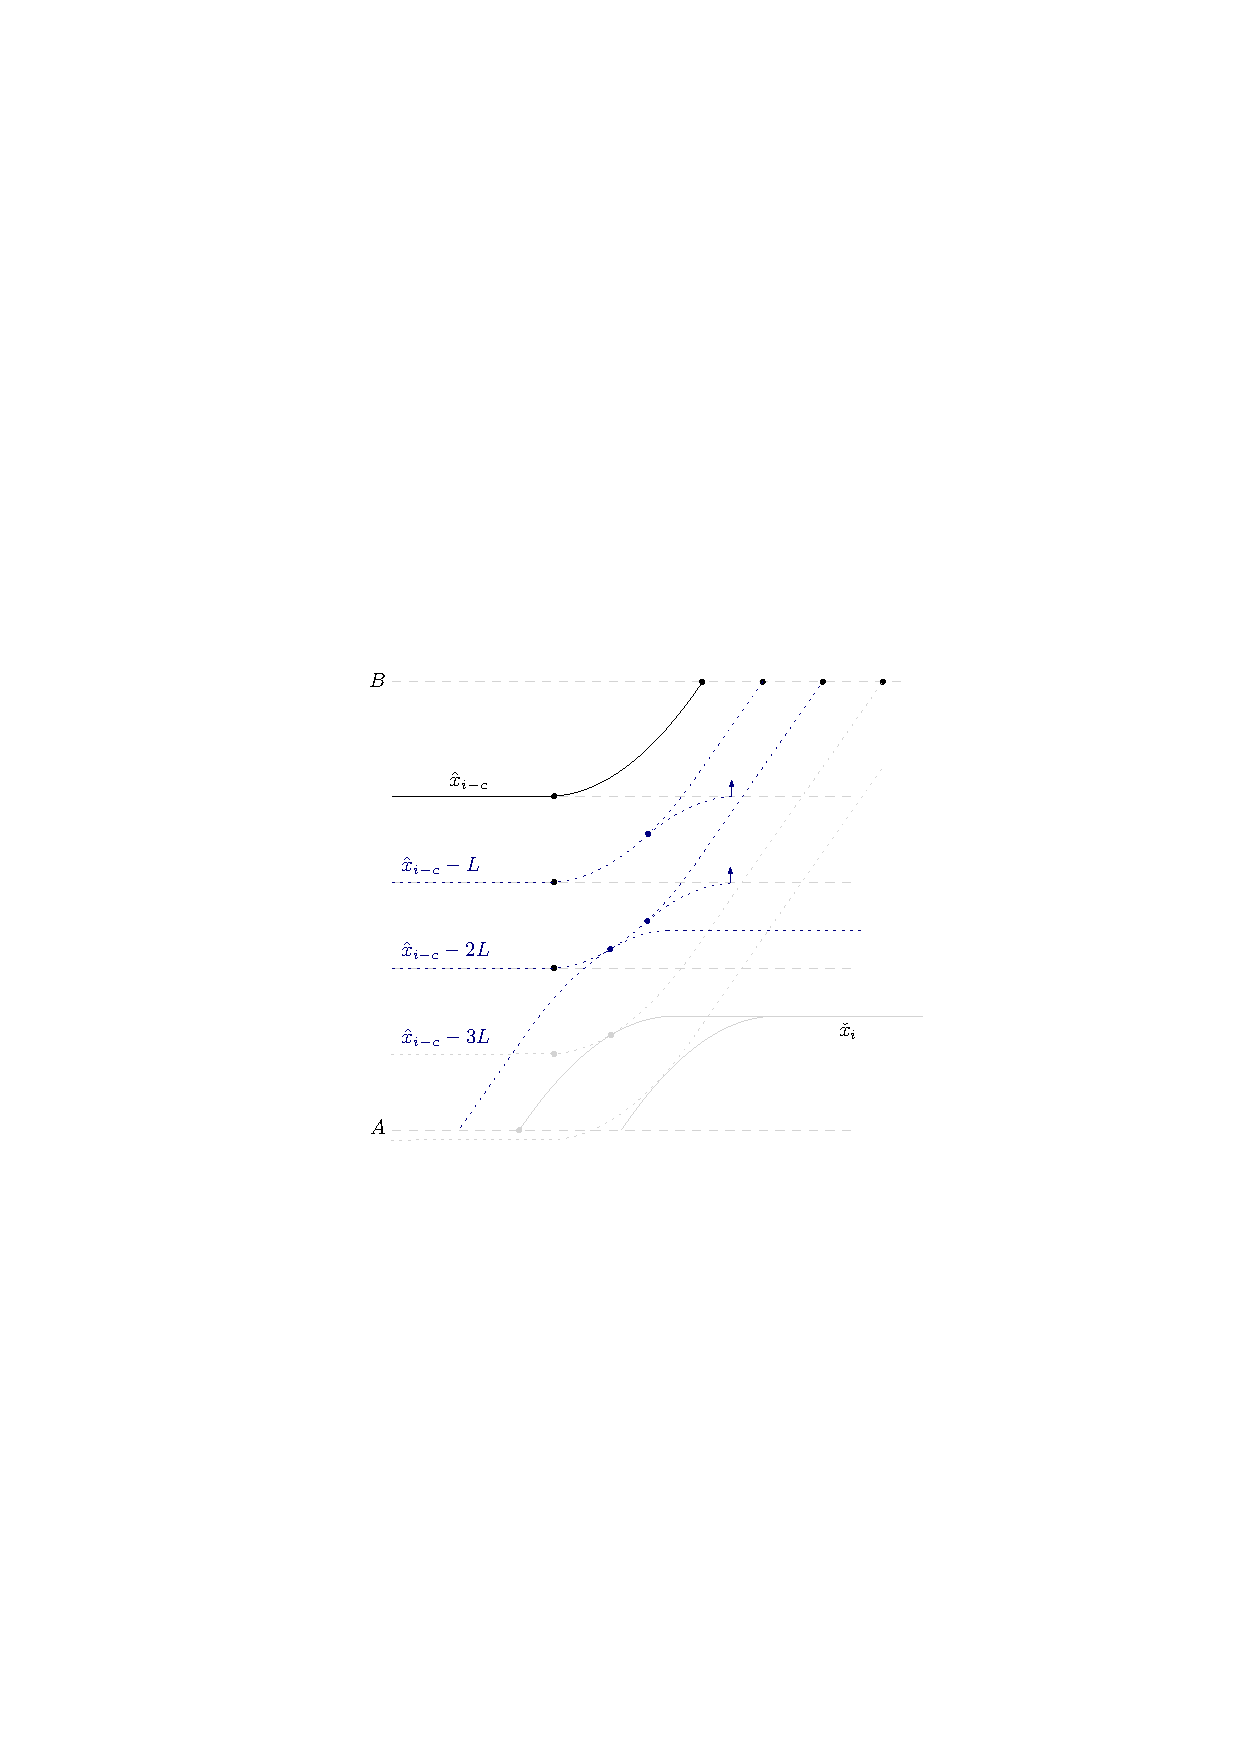
\includegraphics[scale=1]{figures/motion/earliest-arrival}
 \caption{Earliest arrival due to entry order constraint and entry space constraint.}%
\end{figure}



\newpage

\section{Optimal solution for haste objective}

Due to the recursive nature of the problem, we will see that optimal
trajectories possess a particularly simple structure, which enables a simple
computation.

\begin{define}
  Let a trajectory $\gamma \in \mathcal{D}[a, b]$ be called \emph{alternating} if for all
  $t \in [a, b]$, we have
  \begin{align}
    \ddot{\gamma}(t) \in \{-\omega, 0, \bar{\omega}\} \quad \text{ and } \quad
    \ddot{\gamma}(t) = 0 \implies \dot{\gamma}(t) \in \{0, 1\}.
  \end{align}
\end{define}

We now argue that each vehicle's optimal trajectory $x_{i}$ is alternating.
First, consider $x_{1} = x^{*}(a_{1}, b_{1}, \varnothing)$, which is
constructed by joining $x^{1}[x_{1}]$ and $\hat{x}[x_{1}]$ together by smoothing. Observe that both boundaries are alternating by definition. Let
$\gamma_{1}(t) = \min\{x^{1}[x_{1}](t), \hat{x}[x_{1}](t) \}$ be the minimum boundary,
then it is clear that the smoothened $x_{1} = \gamma_{1}^{*}$ must also be
alternating, because we only added a part of deceleration at some interval
$[\xi, \tau]$, which clearly satisfies $\ddot{\gamma}_{1}^{*}(t) = -\omega$ for
$t \in [\xi,\tau]$.
%
Assume that $x_{i-1}$ is alternating, we can similarly argue that $x_{i}$ is
alternating. Again, let
$\gamma_{i}(t) = \min\{\bar{x}[x_{i-1}], \hat{x}[x_{i}](t), x^{1}[x_{i}](t)\}$ be the
minimum boundary. After adding the required decelerations for smoothing, it is
clear that $x_{i} = \gamma^{*}_{i}$ must also be alternating.

\begin{figure}
  \centering
  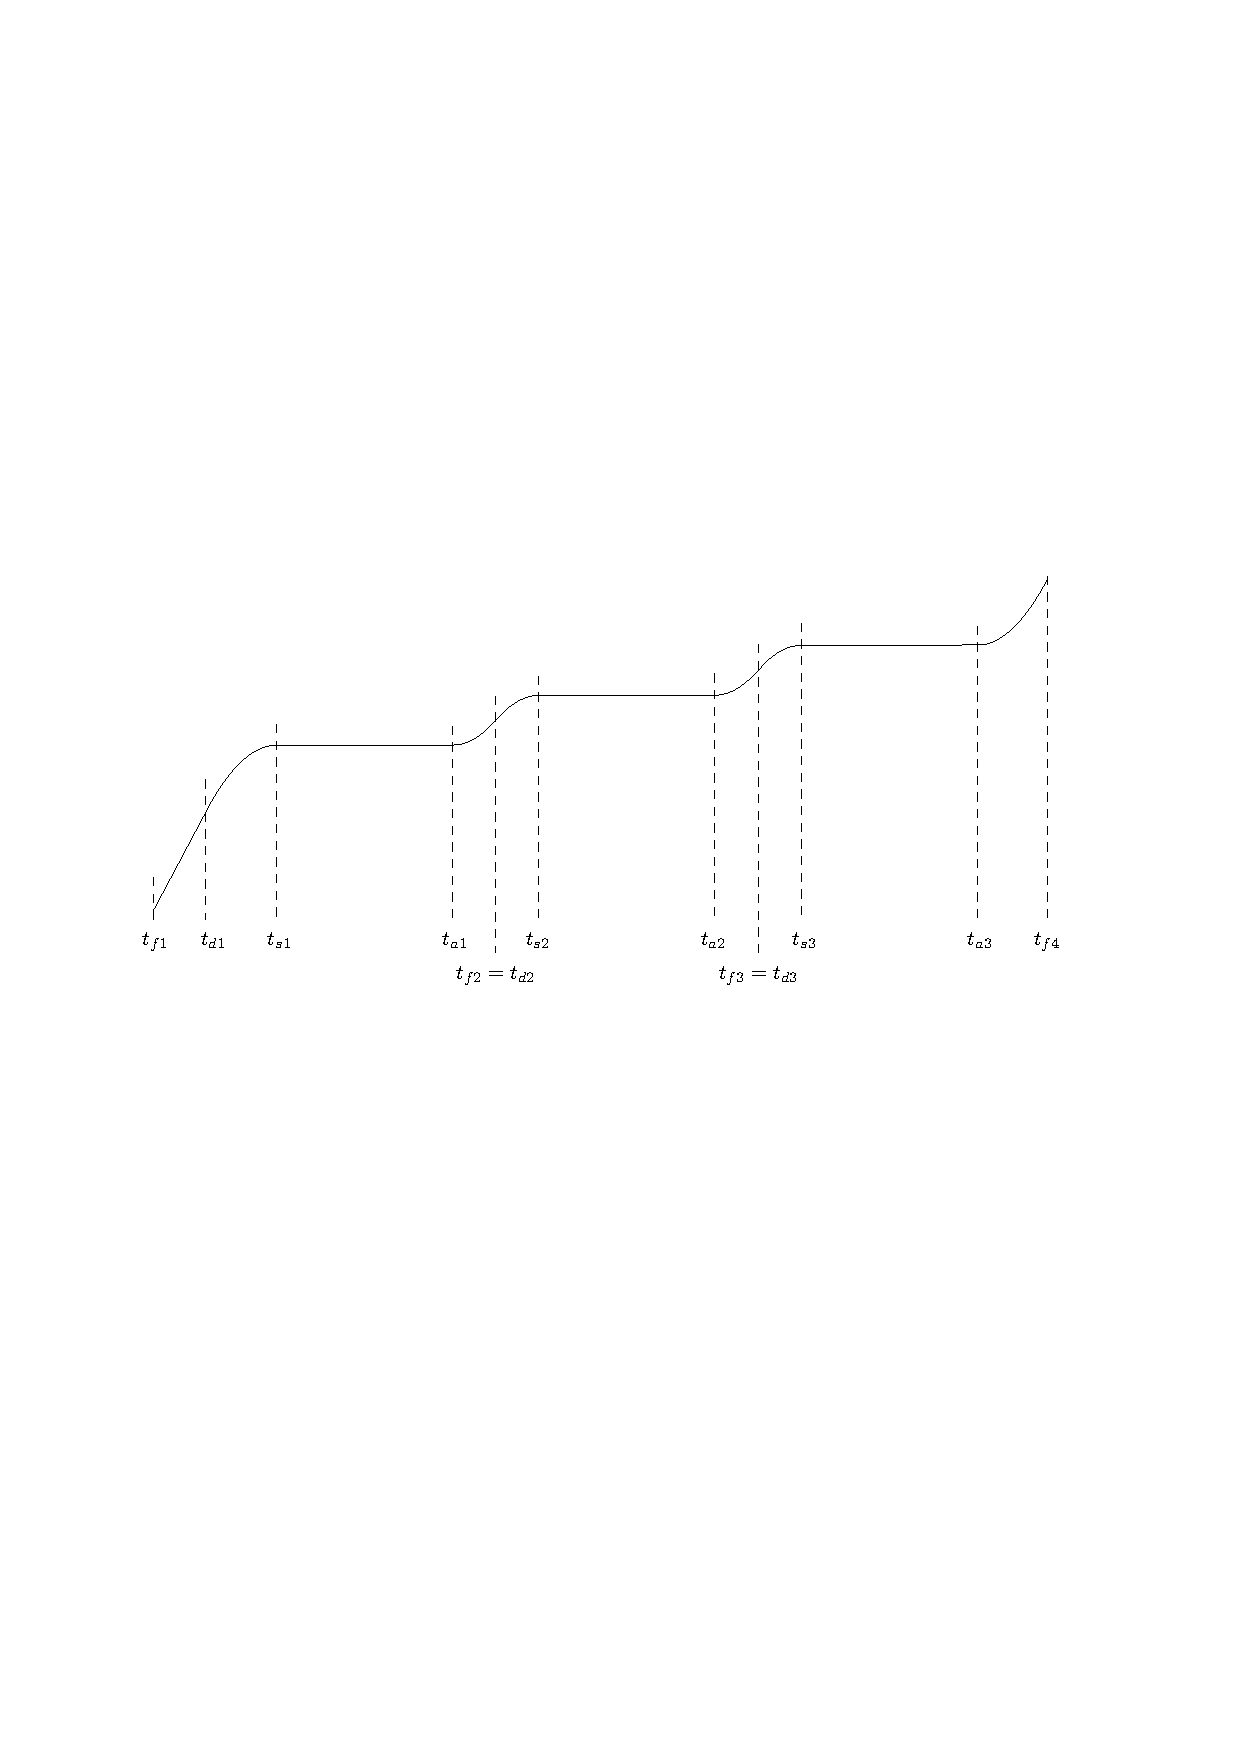
\includegraphics[scale=0.9]{figures/motion/tandem_trajectory}
  \caption{Example of an alternating vehicle trajectory with its defining time
    intervals. The particular shape of this trajectory is due to two leading
    vehicles, which causes the two start-stop \emph{bumps} around the times where these
    leading vehicles depart from the lane.}
  \label{fig:tandem_trajectory}
\end{figure}

Observe that an alternating trajectory $\gamma \in \mathcal{D}[a,b]$ can be described
as a sequence of four types of consecutive repeating phases, see
Figure~\ref{fig:tandem_trajectory} for an example.
%
In general, there exists a partition of $[a,b]$, denoted by
\begin{align*}
  a = t_{f1} \leq t_{d1} \leq t_{s1} \leq t_{a1} \leq t_{f2} \leq t_{d2} \leq t_{s2} \leq t_{a2} \leq \dots \leq t_{f,n+1} = b,
\end{align*}
such that we have the consecutive \emph{alternating intervals}
\begin{alignat*}{3}
  F_{i} &:= [t_{f,i}, t_{d,i}] \quad &\text{ (full speed), } \quad
  S_{i} &:= [t_{s,i}, t_{a,i}] \quad &\text{ (stopped), } \\
  D_{i} &:= [t_{d,i}, t_{s,i}] \quad &\text{ (deceleration), } \quad
  A_{i} &:= [t_{a,i}, t_{f,i+1}] \quad  &\text{ (acceleration), }
\end{alignat*}
%
such that on these intervals, $\gamma$ satisfies
%
\begin{alignat*}{4}
  &\dot{\gamma}(t) = 1 && \text{ for } t \in F_{i} , \quad \quad
  &&\dot{\gamma}(t) = 0 && \text{ for } t \in S_{i} ,\\
  &\ddot{\gamma}(t) = -\omega \quad && \text{ for } t \in D_{i} , \quad \quad
  &&\ddot{\gamma}(t) = \bar{\omega} \quad && \text{ for } t \in A_{i} .
\end{alignat*}

\paragraph{Partial trajectories.}
Next, we will define parameterized functions $x^{f}$, $x^{d}$, $x^{s}$, $x^{a}$
to describe alternating trajectory $\gamma$ on each of these alternating intervals.
%
Given some initial position $p \in [A,B]$, velocity $v \in [0, 1]$, start and end times $a$ and
$b$ such that $a \leq b$ and $v + \bar{\omega}(b - a) \leq 1$, we define the acceleration
trajectory $x^{a}[p, v, a, b] : [a, b] \rightarrow \mathbb{R}$ by setting
\begin{subequations}
\begin{align}
  x^{a}[p,v,a,b](\tau) &:= p + v(\tau - a) + \bar{\omega} (\tau-a)^{2} / 2 , \\
  \dot{x}^{a}[p,v,a,b](\tau) &:= v + \bar{\omega} (\tau - a) .
\end{align}
\end{subequations}
%
Similarly, for $p, v, a, b$ satisfying $a \leq b$ and $v - \omega(b-a) \geq 0$,
let the deceleration trajectory
$x^{d}[p, v, a, b] : [a, b] \rightarrow \mathbb{R}$ be defined as
\begin{subequations}
\begin{align}
  x^{d}[p,v,a,b](\tau) &:= p + v (\tau - a) - \omega (\tau - a)^{2} / 2 , \\
  \dot{x}^{d}[p,v,a,b](\tau) &:= v - \omega (\tau - a) .
\end{align}
\end{subequations}
%
One may notice that $x^{d}$ is essentially the same as the deceleration boundary
$x^{-}$, which we defined in Section~\ref{sec:deceleration-boundary}. However, note that the condition $v - \omega(b-a) \geq 0$ restricts the domain such that we do not need the clipping operation. Furthermore, the parameterization of $x^{d}$ will be more convenient in the next section.

We use the following notation for trajectories with constant minimum or maximum
speed. We write $x^{s}[p, a, b](\tau) \equiv p$, with domain $[a,b]$, to model a stopped
vehicle and let $x^{f}[p, a, b](\tau) = (p + \tau - a, 1)$ model a vehicle that drives
at full speed, also with domain $[a,b]$.


\subsection{Connecting partial trajectories}

It can be shown that the smoothing procedure introduces a part of deceleration
only between the four pairs of partial trajectories
\begin{align*}
    x^{a} \rightarrow x^{a} , \quad \quad
    x^{a} \rightarrow x^{s} , \quad \quad
    x^{f} \rightarrow x^{a} , \quad \quad
    x^{f} \rightarrow x^{s} .
\end{align*}
We will use these results to characterize optimal trajectories for our optimal
control problem.

\begin{lemma}[$x^{f} \rightarrow x^{s}$]
  Let $x^{f}[p, a, b]$ and $x^{s}[q, c, d]$ be two trajectories. Considering
  $\tau_{1}$ and $\tau_{2}$ as variables in the equation
  \begin{align*}
    x^{d}[x^{f}[p, a, b](\tau_{1}), \tau_{1}, \tau_{2}](\tau_{2}) = x^{s}[q, c, d](\tau_{2}) ,
  \end{align*}
  it has solution
  $\tau_{2} = q - p + a + 1/2\omega$ and $\tau_{1} = \tau_{2} - 1/\omega$, whenever
  $\tau_{1} \in [a, b]$ and $\tau_{2} \in [c, d]$.
\end{lemma}
\begin{proof}
  The expanded system of state equations is given by
  \begin{align*}
    \begin{cases}
      p + \tau_{1} - a + (\tau_{2} - \tau_{1}) - \omega(\tau_{2} - \tau_{1})^{2} / 2 = q , \\
      1 - \omega(\tau_{2} - \tau_{1}) = 0 .
    \end{cases}
  \end{align*}
  The second equation yields $\tau_{2} - \tau_{1} = 1/\omega$, which after
  substituting back in the first equation yields
  $p - a + \tau_{2} - 1/2\omega - q = 0$, from which the stated solution
  follows.
\end{proof}


\begin{figure}
\centering
\begin{minipage}{.45\textwidth}
  \centering
  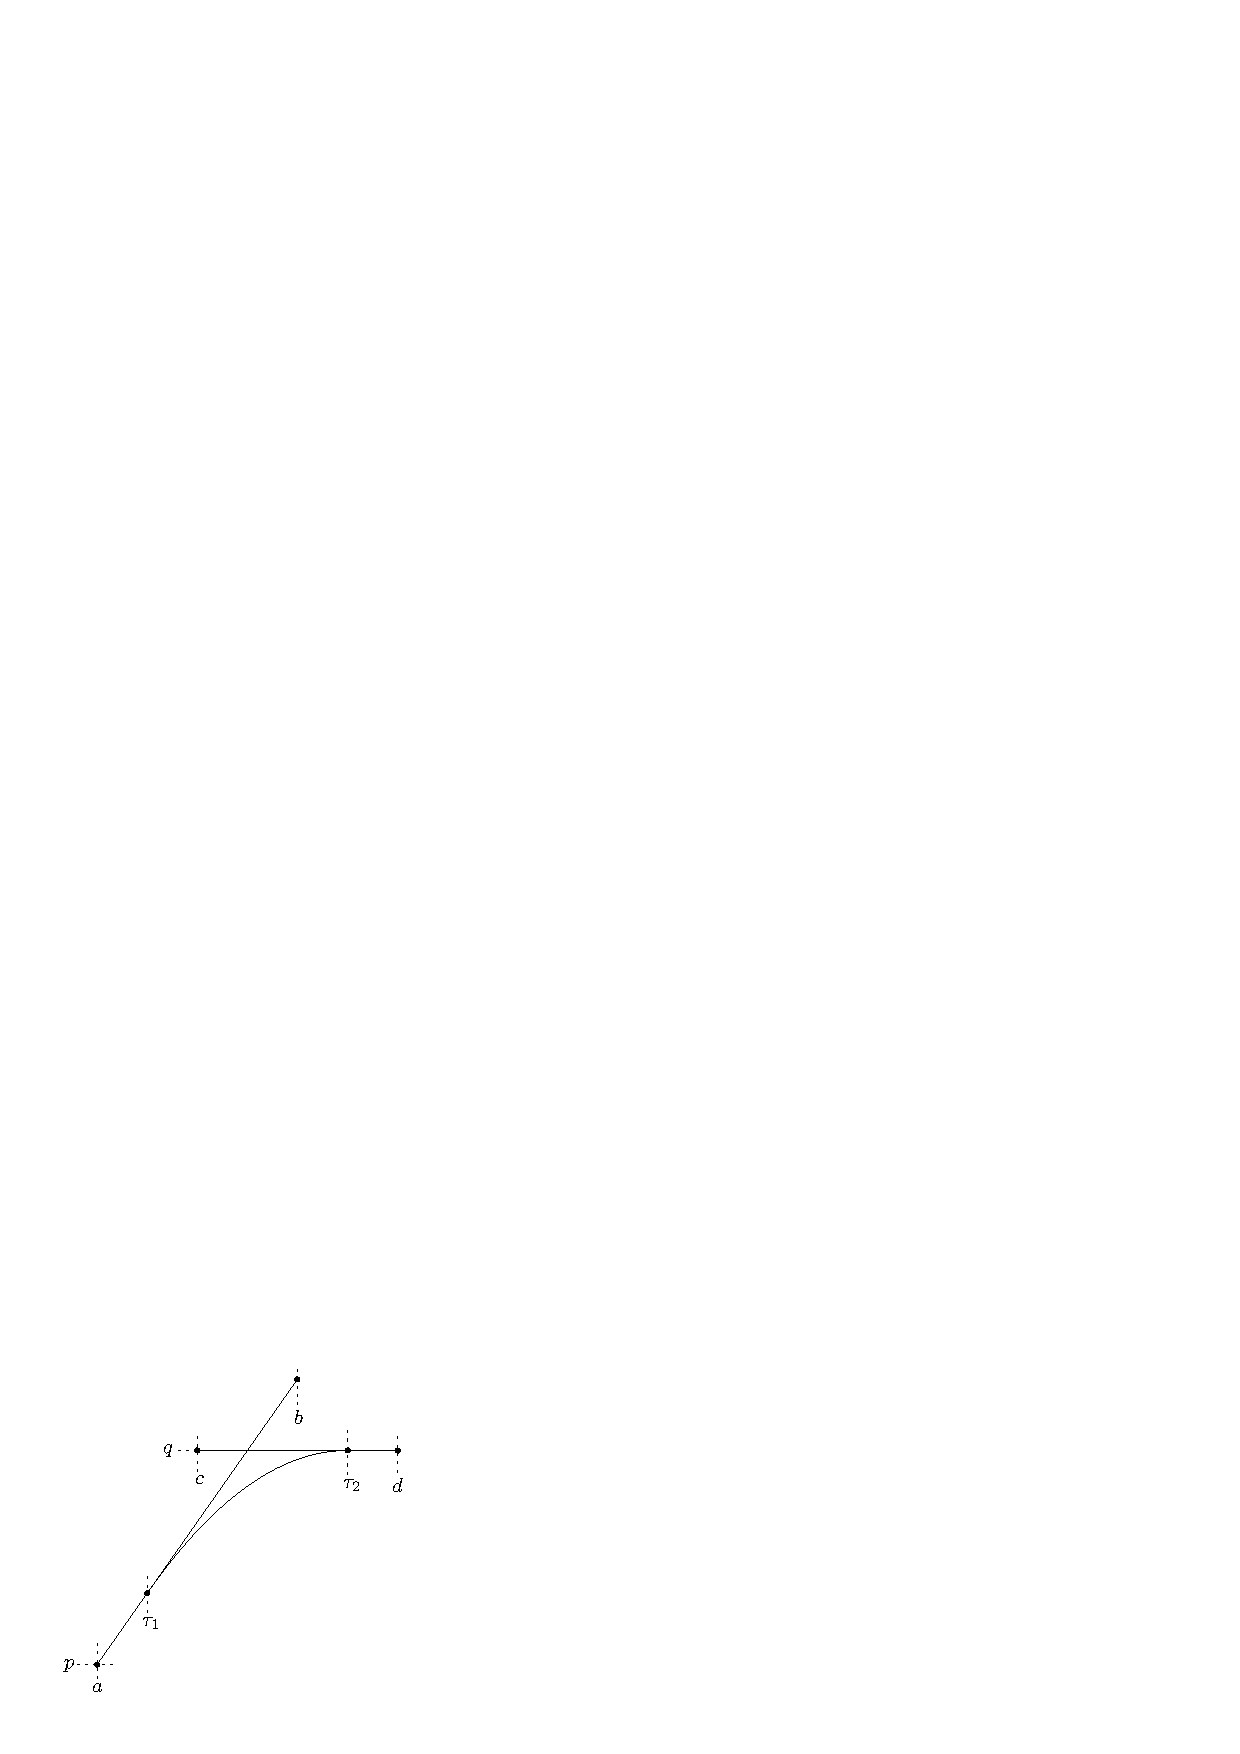
\includegraphics[width=0.9\linewidth]{figures/motion/lemma_full_still}
  \captionof{figure}{$x^{f} \rightarrow x^{s}$}
  \label{fig:full_still}
\end{minipage}%
\hspace{1.0em}
\begin{minipage}{.45\textwidth}
  \centering
  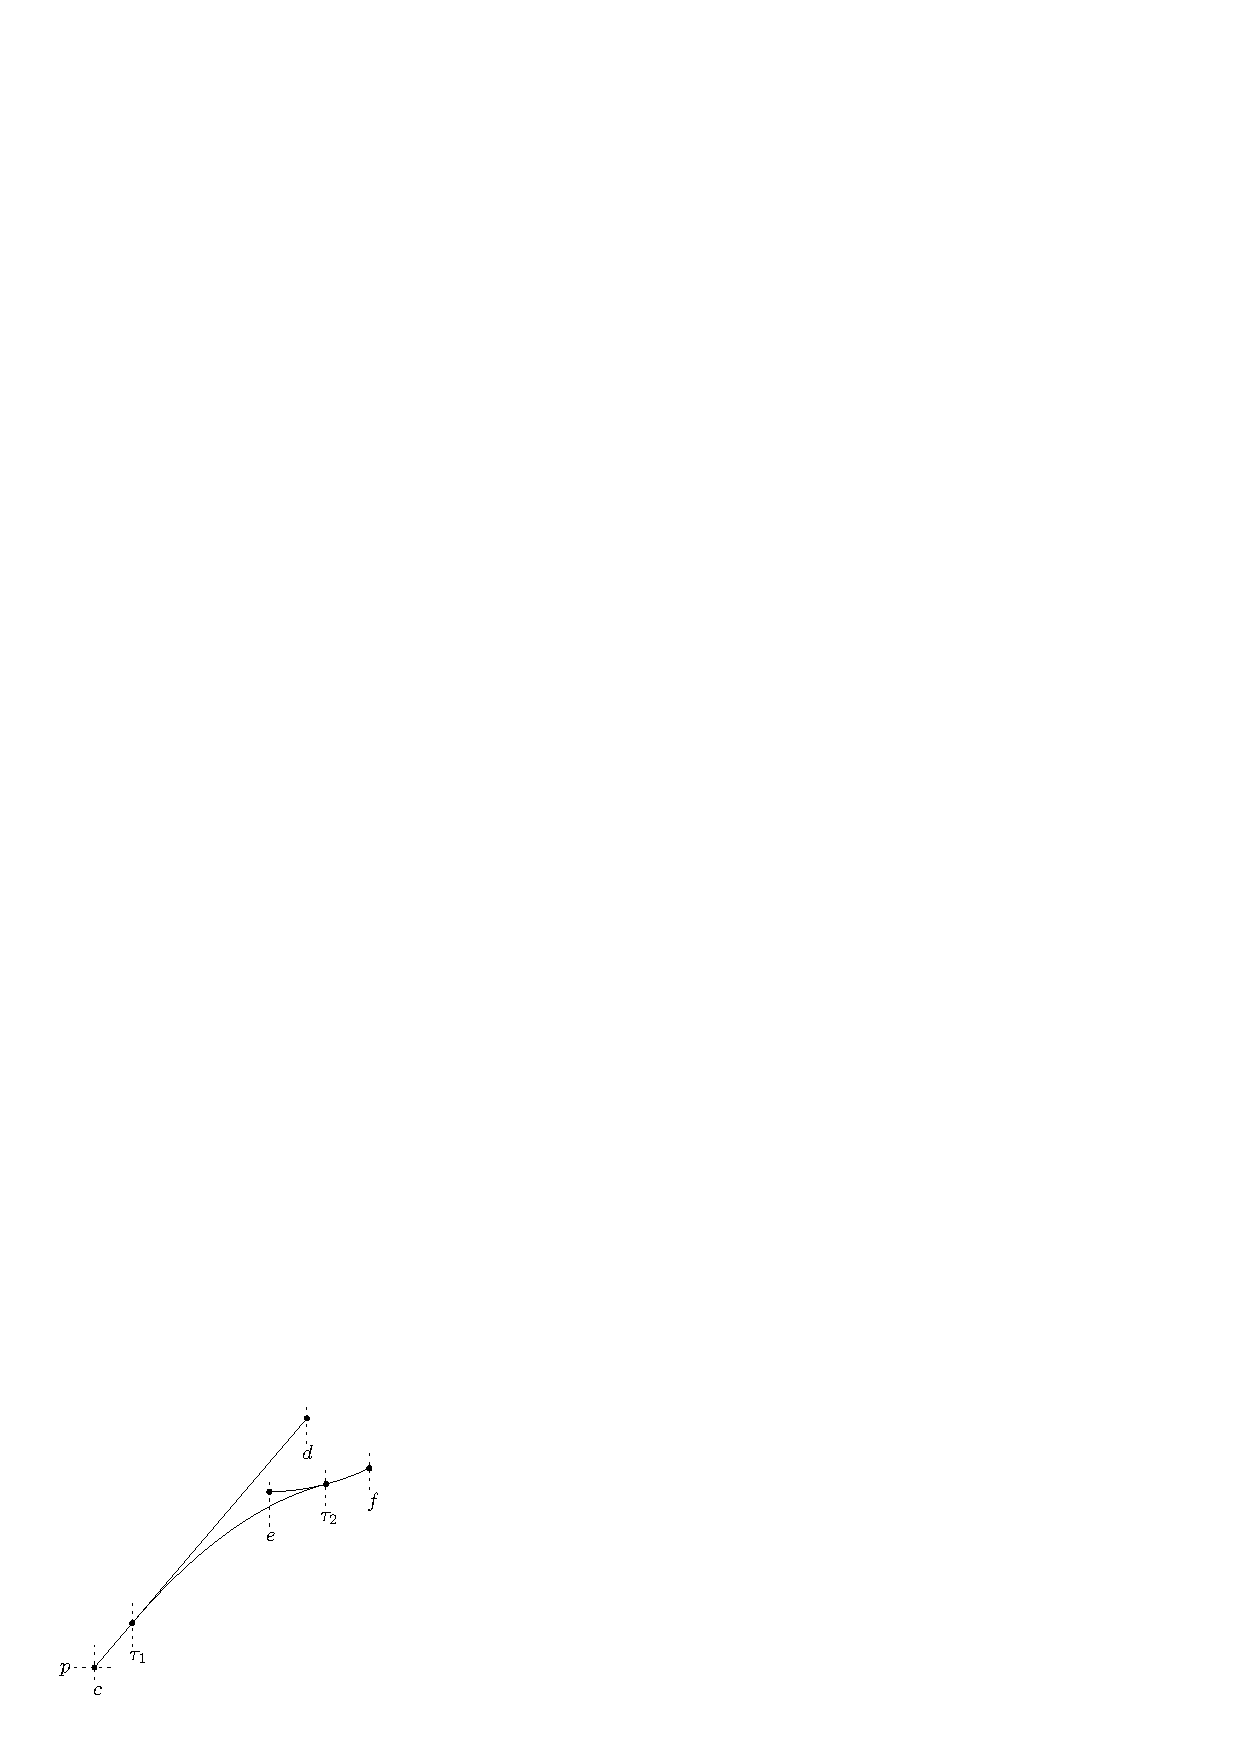
\includegraphics[width=0.9\linewidth]{figures/motion/lemma_full_acc}
  \captionof{figure}{$x^{f} \rightarrow x^{a}$}
  \label{fig:full_acc}
\end{minipage}
\end{figure}

To keep the expressions for the case of joining $x^{f} \rightarrow x^{a}$ a
little bit simpler, we first consider a full line joining to a acceleration
trajectory of full length $1/\omega$.

\begin{lemma}
  \label{lemma:line_acc}
  Consider some full acceleration trajectory $x^{a}[(p, 0), a, a+1/\omega]$ and the
  line through $(\lambda, 0)$ with slope 1. Whenever $\lambda$, which can be
  interpreted as a time epoch, satisfies $\lambda \in [a-p-1/2\omega, a-p+1/2\omega]$, then the equation
  \begin{align*}
    x^{+}[(p, 0), a, a+1/\omega](\tau) = x^{d}[(q, 1), q + \lambda, q + \lambda + 1/\omega](\tau) ,
  \end{align*}
  with $\tau$ and $q$ considered as variables, has a unique solution
  \begin{align*}
    \tau &= a + 1/\omega - \sqrt{\frac{a - p + 1/2\omega - \lambda}{\omega}} , \\
    q &= 2\tau - a - 1/\omega - \lambda ,
  \end{align*}
  so the joining deceleration is given by $x^{d}[(q,1), q + \lambda, \tau]$
\end{lemma}
\begin{proof}
  First of all, the expanded system of state equations is given by
  \begin{align*}
    \begin{cases}
    p + \omega (\tau - a)^{2}/2 = q + (\tau - q - \lambda) - \omega (\tau - q - \lambda)^{2}/2 , \\
    \omega(\tau - a) = 1 - \omega(\tau - q - \lambda) .
      \end{cases}
  \end{align*}
  We use the second equation to express $q$ in terms of $\tau$, which yields
  \begin{align*}
    q = 2\tau - 1/\omega -a - \lambda ,
  \end{align*}
  which we substitute in the first equation to derive the equation
  \begin{align*}
    \omega \tau^{2}  - 2 (1 + \omega a) \tau + \omega a^{2} + a + p + \lambda + 1/2\omega = 0 .
  \end{align*}
  This is a quadratic equation in $\tau$, with solutions
  \begin{align*}
    \tau = a + 1/\omega \pm \sqrt{\frac{a - p + 1/2\omega - \lambda}{\omega}} ,
  \end{align*}
  of which only the smallest one is valid, because $\tau \leq a + 1/\omega$.
  Furthermore, we see that $\tau$ is defined as a real number when
  \begin{align*}
    a - p + 1/2\omega - \lambda \geq 0 \iff \lambda \leq a - p + 1/2\omega .
  \end{align*}
  The other requirement is that $\tau \geq a$, which is equivalent to
  \begin{align*}
    1/\omega \geq \sqrt{\frac{a - p + 1/2\omega - \lambda}{\omega}} \iff
    % 1/\omega \geq a - p - \lambda + 1/2\omega \iff
    \lambda \geq a - p - 1/2\omega .
  \end{align*}
\end{proof}

\begin{lemma}[$x^{f} \rightarrow x^{a}$]
Consider partial trajectories $x^{f}[p, c, d]$ and $x^{a}[x, e, f]$.
\end{lemma}
\begin{proof}
  First of all, observe that $x^{f}[p, c, d]$ lies on the line with slope 1
  through $(\lambda, 0) := (c - p, 0)$ and $x^{a}[x, e, f]$ lies on the full
  acceleration curve
  $x^{a}[(x_{1} - x_{2}^{2}/(2\omega) , 0), e - x_{2}/\omega, e - x_{2}/\omega + 1/\omega]$, see
  Figure~\ref{fig:full_acc}.
  %
  Now apply Lemma~\ref{lemma:line_acc} to $p = x_{1} - x_{2}^{2}/(2\omega)$,
  $a = e - x_{2}/\omega$ and $\lambda = c - p$ yields some solutions $\tau$ and $q$.
  %
  Let $\tau_{2} := \tau$ and let $\tau_{1}$ denote the time where the line and
  $x^{a}$ join, given by $\tau_{1} = \lambda + q$. Now we simply check whether this
  solution is also feasible for the smaller trajectories. We must have
  $\tau_{1} \in [c, d]$ and $\tau_{2} \in [e, f]$.
\end{proof}


\begin{lemma}
  \label{lemma:acc_hline}
  Consider the acceleration trajectory $x^{a}[(p, 0), a, b]$ and the horizontal
  line through $(0, q)$. Let $\tau_{1} = a + \sqrt{(q-p)/\omega}$ and
  $\tau_{2} = a + 2\sqrt{(q-p)/\omega}$. If $\tau_{1}$ satisfies
  $\tau_{1} \in [a, b]$, then both trajectories are joined by deceleration
  trajectory $x^{d}[x^{a}[(p, 0), a, b](\tau_{1}), \tau_{1}, \tau_{2}]$
\end{lemma}
\begin{proof}
  Consider the following equation
  \begin{align*}
    x^{d}[x^{a}[(p, 0),a,b](\tau_{1}), \tau_{1}, \tau_{2}](\tau_{2}) = (q, 0) .
  \end{align*}
  %
  The expanded system of state equations is given by
  \begin{align*}
    \begin{cases}
      p + \omega (\tau_{1} - a)^{2}/2 + (\omega(\tau_{1} - a)) (\tau_{2} - \tau_{1}) - \omega(\tau_{2} - \tau_{1})^{2}/2 = q , \\
      \omega(\tau_{1} - a) - \omega(\tau_{2} - \tau_{1}) = 0 .
    \end{cases}
  \end{align*}
  From the second equation, we derive $\tau_{1} - a = \tau_{2} - \tau_{1}$.
  Plugging this back in the first equation yields the quadratic equation
  $p + \omega(\tau_{1} - a)^{2} = q$ with solutions
  $\tau_{1} = a \pm \sqrt{(q-p)/\omega}$, of which only the larger one is valid.
  Finally, the second equation gives $\tau_{2} = 2\tau_{1} - a$.
\end{proof}

\begin{lemma}[$x^{a} \rightarrow x^{s}$]
  Consider partial trajectories $x^{a}[x, c, d]$ and $x^{s}[q, e, f]$.
\end{lemma}
\begin{proof}
  Observe that $x^{a}[x, c, d]$ lies on the full acceleration curve
  $x^{a}[(x_{1} - x_{2}^{2}/(2\omega), 0), c - x_{2}/\omega, c - x_{2}/\omega + 1/\omega]$.
  Hence, we can apply Lemma~\ref{lemma:acc_hline} with
  $p=x_{1} - x_{2}^{2}/(2 \omega)$, $a = c - x_{2}/\omega$, which yields some
  solutions $\tau_{1}$ and $\tau_{2}$, which are feasible solutions if
  $\tau_{1} \in [c, d]$ and $\tau_{2} \in [e, f]$.
\end{proof}

\begin{lemma}
  Consider full acceleration trajectories $x^{a}[(p, 0), a, b]$ and
  $x^{a}[(q, 0), c, d]$.
\end{lemma}
\begin{proof}
  Consider the equation
  \begin{align*}
    x^{d}[x^{a}[(p, 0), a, b](\tau_{1}), \tau_{1}, \tau_{2}](\tau_{2}) = x^{a}[(q, 0), c, d](\tau_{2}) ,
  \end{align*}
  expanded to the system of equations
  \begin{align*}
    \begin{cases}
      p + \omega(\tau_{1} - a)^{2}/2 + \omega(\tau_{1} - a)(\tau_{2} - \tau_{1}) - \omega(\tau_{2} - \tau_{1})^{2}/2 = q + \omega(\tau_{2} - c)^{2}/2 , \\
      \omega(\tau_{1} - a) + \omega(\tau_{2} - \tau_{1}) = \omega(\tau_{2} - c) .
    \end{cases}
  \end{align*}
\end{proof}

\begin{lemma}[$x^{a} \rightarrow x^{a}$]
  Consider partial trajectories $x^{a}[x, a, b]$ and $x^{a}[y, c, d]$.
\end{lemma}
\begin{proof}

\end{proof}

\subsection{Algorithm}

Put everything together into pseudocode.

\begin{algorithm}
  \caption{Computing connecting deceleration for alternating trajectories.}
    \label{alg:connecting}
    \begin{algorithmic}
      \State Let $i$ such that $I_{i}$ is the latest such that $t_{1} < I_{i}$.
      \State Let $j$ such that $I_{j}$ is the earliest such that $t_{1} > I_{j}$.
    \end{algorithmic}
\end{algorithm}


\pagebreak
\section{Network planning problem}

Due to the second-order boundary conditions
$\dot{x}_{i}(a_{i}) = \dot{x}_{i}(b_{i}) = 1$, the feasibility of the lane
planning problem is completely characterized in terms of its schedule times.
%
We will show that it is precisely this property that us to construct a network
consisting of individual lanes, connected at intersections.
%
The fact that intersections are shared among multiple lanes naturally gives rise to some collision-avoidance constraints.
%
We will see that the feasibility of finding collision-free trajectories can be
stated completely in terms of schedule times, which essentially means that we do
not need to worry about vehicle dynamics at all.

\paragraph{Network topology.}

We will use the lane model to build a simple network model. The network model is
based on a directed graph $(\bar{V},E)$ with nodes $\bar{V}$ and arcs $E$, which
we will use to encode the possible routes.
%
Nodes with no incoming arcs are \textit{entrypoints} and nodes with no outgoing
arcs are \textit{exitpoints}.
%
We use $V$ to denote the set of \textit{intersections}, which are nodes with
in-degree at least two.
%
Let $\mathcal{R}$ denote the index set for routes, then each $r \in \mathcal{R}$
corresponds to the route
\begin{align*}
  \bar{V}_{r} = (v_{r}(0), v_{r}(1), \dots, v_{r}(m_{r}), v_{r}(m_{r}+1)) ,
\end{align*}
%
where we require $v_{r}(0)$ to be an entrypoint and $v_{r}(m_{r}+1)$ to be an
exitpoint. Furthermore, we use
$V_{r} = \bar{V}_{r} \setminus \{ v_{r}(0), \, v_{r}(m_{r}+1) \}$ to denote the
intersections on this route.
%
Let $E_{r} \subset E$ denote the set of edges that make up $V_{r}$.
%
We require that routes are \emph{edge-disjoint}, which is made precise in the
following assumption.

\begin{assump}\label{assump:disjoint-routes}
  For every distinct routes $p,q \in \mathcal{R}$ such that $p \neq q$, we
  assume $E_{p} \neq E_{q}$.
\end{assump}

This assumption ensures that each route $\bar{V}_{r}$ can be modeled by
connecting a sequence of lanes together, with some \emph{intersection areas} of
some fixed size $W$ in between them, see Figure~\ref{fig:intersections}.
%
Hence, we set the longitudinal start and end position of each lane model as
follows. Let $d(v, w)$ denote the length of edge $(v,w) \in E_{r}$, then we
recursively define
\begin{subequations}
\begin{align}
  A_{r1} &= 0 , \\
  A_{rk} &= B_{r,k-1} + W + L , \\
  B_{rk} &= A_{rk} + d(v_{r}(k-1), v_{r}(k)) ,
\end{align}
\end{subequations}
for each $k \in \{1, \dots, m_{r} + 1\}$.


\begin{figure}
  \centering
  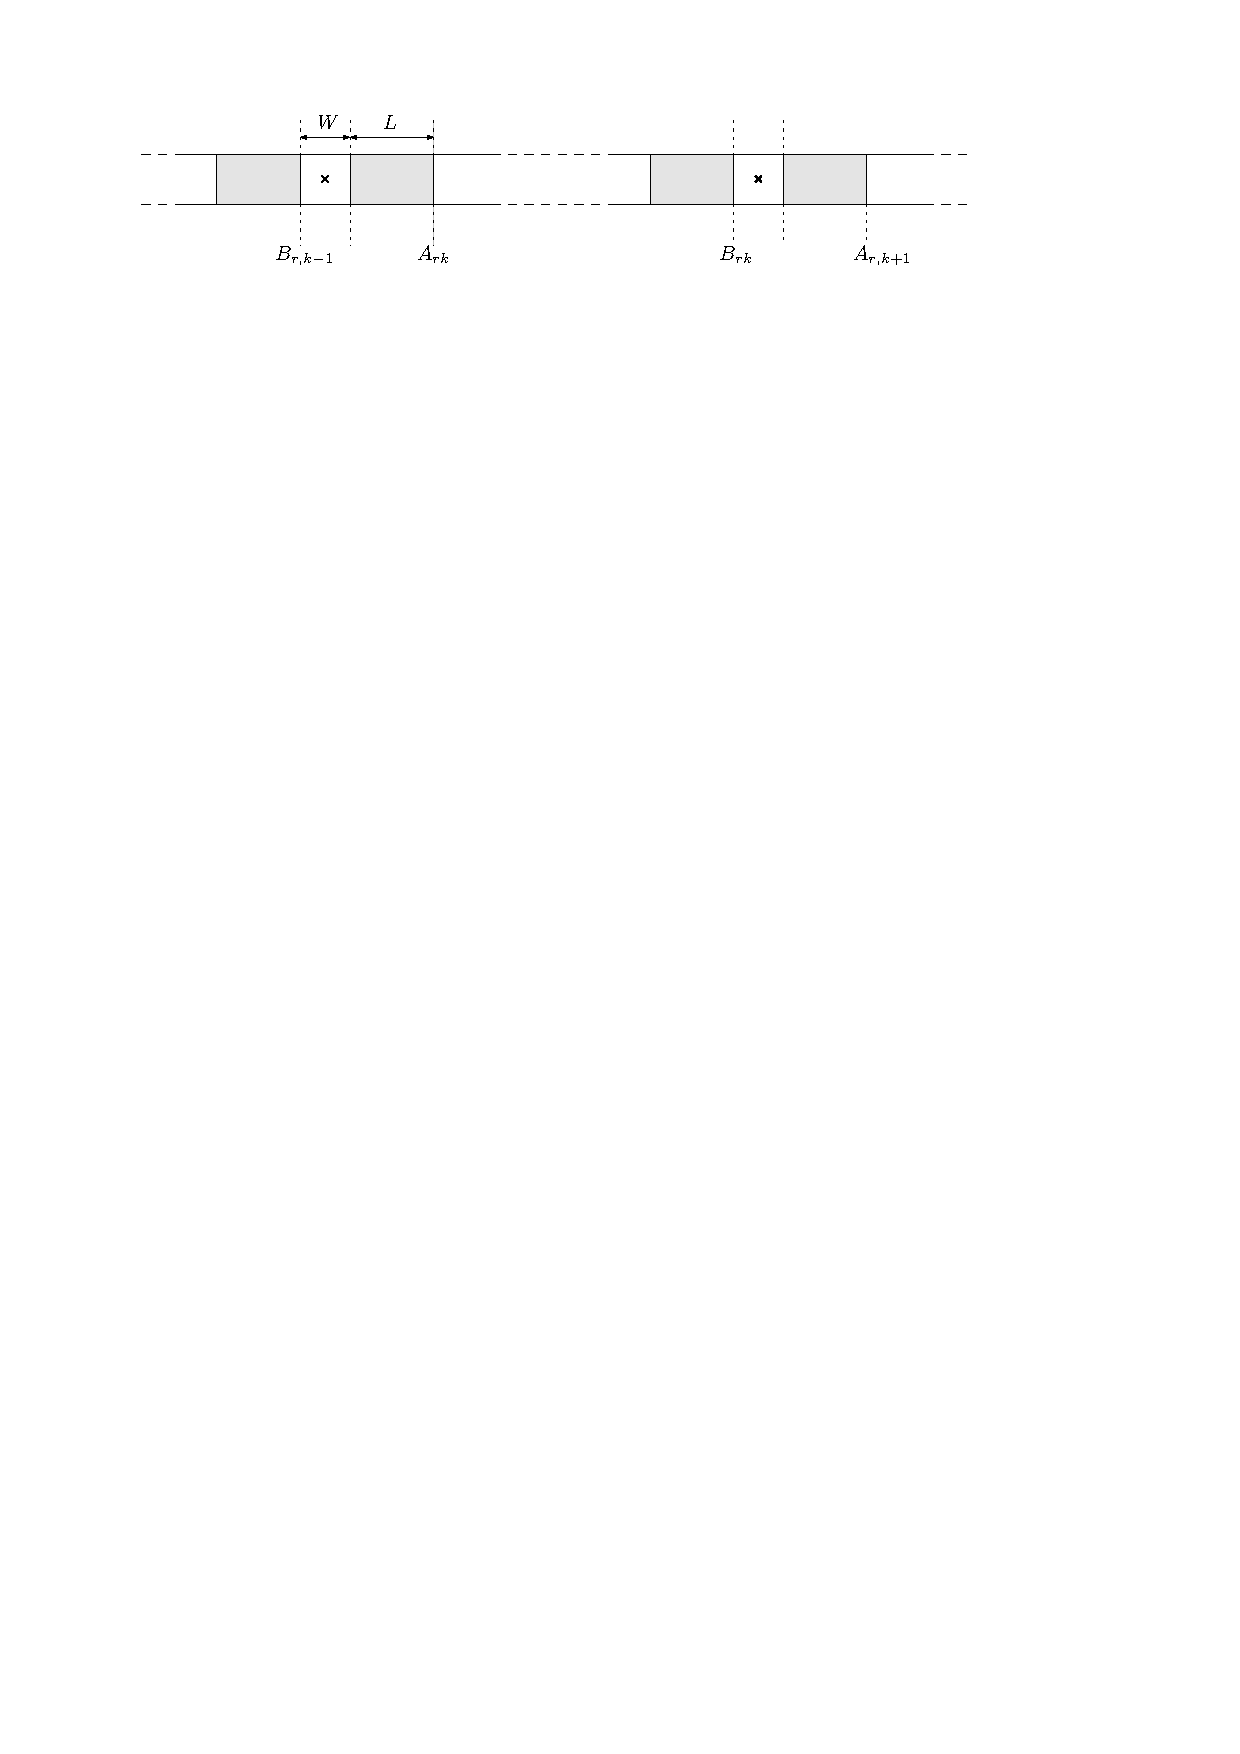
\includegraphics[scale=1]{figures/motion/intersection}
  \caption{Illustration of how the individual lane models are connected to form
    a route with intersections, marked with a little cross. The four shaded
    rectangles illustrate four possible vehicle positions. The length of the
    intersection is $W$. The longitudinal positions $A_{rk}$ and $B_{rk}$ denote
    the start and end, respectively, of the $k$th lane on route $r$.}%
  \label{fig:intersections}
\end{figure}

\paragraph{Network scheduling.}
Introduce the global trajectory planning problem by defining the
collision-avoidance constraints.
Mention that this problem can be solved at once, by using direct transcription.
%
Show that the bilevel formulation decomposes into a (combinatorial) scheduling
problem.

Assumption~\ref{assump:disjoint-routes} ensures that the order of vehicles on
each lane is completely determined by the order of vehicles on the corresponding
lane.

Instead of schedule times $a_{i}$ and $b_{i}$, we are now going to use crossing
times $y_{i}$.

{\color{Navy} Occupancy time slot scheduling}


\section{Discussion}

There are different ways of relaxing the second-order constraints that could be
studied.
%
The interesting question is whether feasibility can still be easily characterized.
%
Instead of fixing the speed to be maximal at entry and exit, we could
require, for example, that the speed is bounded from below, i.e.,
\begin{align}
  \label{eq:1}
  \eta \leq \dot{x}(a) \leq 1 \quad \text{ and } \quad \eta \leq \dot{x}(b) \leq 1 ,
\end{align}
for some $\eta > 0$.

\newpage
\appendix
\section{Miscellaneous}

\begin{lemma}\label{lemma:inf-continuous}
  Let $f : X \times Y \rightarrow \mathbb{R}$ be some continuous function. If
  $Y$ is compact, then the function $g : X \rightarrow \mathbb{R}$, defined as
  $g(x) = \inf \{ f(x,y) : y\in Y\}$, is also continuous.
\end{lemma}

\begin{lemma}\label{lemma:levelset}
  Let $f :\mathbb{R}^{n} \rightarrow \mathbb{R}^{m}$ be continuous and
  $y \in \mathbb{R}^{m}$, then the level set $N := f^{-1}(\{ y \})$ is a closed
  subset of $\mathbb{R}^{n}$.
\end{lemma}
\begin{proof}
  For any $y' \neq y$, there exists an open neighborhood $M(y')$ such that
  $y \notin M(y')$. The preimage $f^{-1}(M(y'))$ is open by continuity.
  Therefore, the complement
  $N^{c} = \{ x : f(x) \neq y \} = \cup_{y' \neq y} f^{-1}(\{y'\}) = \cup_{y' \neq y} f^{-1}(M(y'))$
  is open.
\end{proof}

\end{document}

% to enable the minted package
% Local Variables:
% TeX-command-extra-options: "-shell-escape"
% End:
